\chapter{Implementación del software\label{sec:Implementacion_soft}}

Una vez finalizado el soporte físico del sistema será necesario implementar a nivel de software todas las funciones deseadas.

El sistema está compuesto por \textbf{tres microcontroladores}, cada uno de ellos con sus propias características y métodos de programación. A lo largo de este capítulo se explicará con detenimiento el software utilizado individualmente para ellos así como los distintos entornos de desarrollo (\acrshort{IDE}) necesarios.

Los distintos elementos se presentarán siguiendo el mismo orden que la información que se desea adquirir. Este es:
\textbf{$$\text{ADS} \Rightarrow \text{Microcontrolador} \Rightarrow \text{Interfaz inalámbrica} \Rightarrow \text{PC}$$}

\section{Microcontrolador STM32F4\label{sec:Software_micro}}

Debido a la complejidad de los microcontroladores de la familia STM32, los desarrolladores han dedicado su tiempo y esfuerzo en crear herramientas que faciliten su programación. Estas herramientas llamadas \textbf{\acrshort{IDE}} contienen una \textbf{recopilación de funciones}, \textbf{utilidades y ejemplos} que simplifican sensiblemente el proceso de diseño e implementación del software que ejecutará el microcontrolador.

Es tan grande la comunidad de desarrolladores que hay detrás del STM que numerosas empresas han visto como una oportunidad de negocio la creación de un \acrshort{IDE} propietario.

\clearpage

\begin{figure} [h]
    \centering
    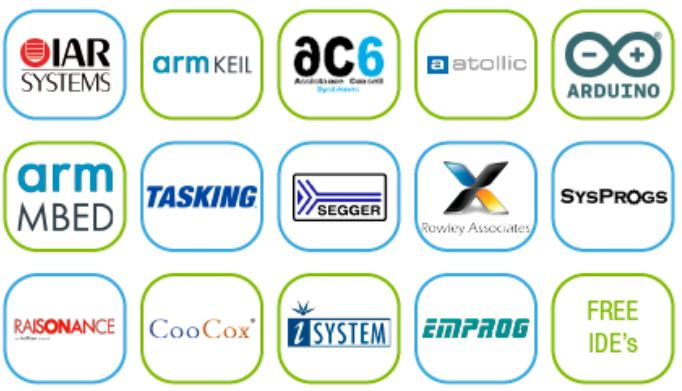
\includegraphics[width=13cm]{STM32_IDEs}
    \caption{IDEs alternativos disponibles \cite{STM32_IDEs}}
    \label{fig:STM32_IDEs}
\end{figure}

La figura \ref{fig:STM32_IDEs} muestra algunos entornos de desarrollo recomendados por el fabricante en su propia página web. Como se puede apreciar se hace distinción entre las opciones comerciales (azul) y las gratuitas (verde).

Uno de los \textbf{objetivos} de este proyecto era \textbf{utilizar Software Libre} en la medida de lo posible. Por ese motivo se probaron algunas de las alternativas presentes en la imagen anterior dando preferencia a aquellas basadas en Oracle como ``System Workbench for STM32'' (AC6). A continuación se presentan algunas de las utilizadas al comienzo del proyecto junto con sus características y el motivo de su descarte:
\begin{itemize}
   \item \textbf{CooCox}\\
   Presenta muchos ejemplos prácticos pero su interfaz es muy lenta. Necesita demasiado tiempo para iniciar.
   \item \textbf{Arduino}\\
   Fase muy temprana de desarrollo.
   \item \textbf{System Workbench for STM32}
   \\Buena comunidad pero incompatible con las herramientas de STM.
\end{itemize}

\begin{figure} [h]
    \centering
    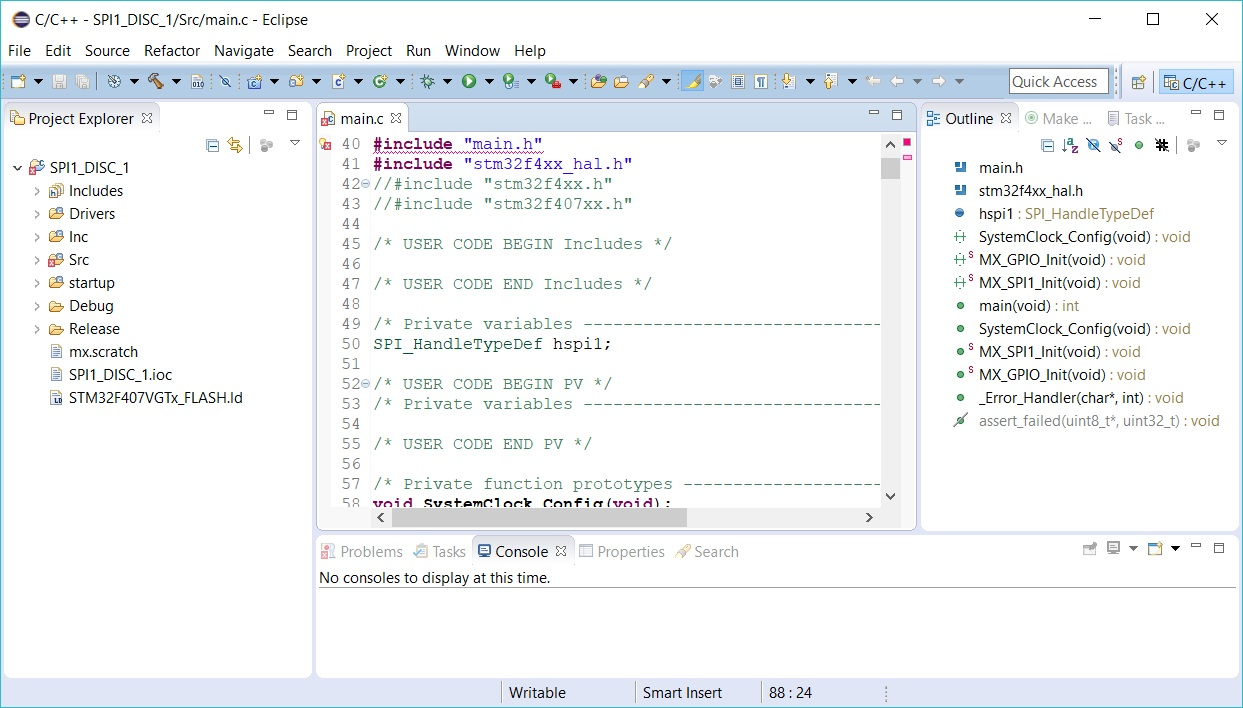
\includegraphics[width=12cm]{Alternative_IDE}
    \caption{Ejemplo de IDE alternativo basado en Oracle (System Workbench for STM32)}
    \label{fig:Alternative_IDE}
\end{figure}

Finalmente se optó por \textbf{armKeil} ya que tiene una gran \textbf{cantidad de ejemplos y librerías descargables} desde la propia interfaz, contiene un gran número de \textbf{funciones adicionales} y la compatibilidad con las herramientas de STM es muy buena. Aunque en la figura \ref{fig:STM32_IDEs} aparece entre las alternativas gratuitas se debe destacar que cuenta con dos versiones: una gratuita que permite realizar proyectos básicos y otra comercial, destinada a aplicaciones de mayor envergadura. La \textbf{limitación de la versión gratuita} consiste en forzar un tamaño máximo de programa de \textbf{32KB}. Si el código a compilar supera dicha longitud directamente no compilará.

\subsection{Configuración inicial\label{sec:Configuracion_micro}}

Aunque Keil permite comenzar un proyecto utilizando como base algunos de los ejemplos que contiene, la configuración de las características del microcontrolador (reloj, interfaces, etc.) puede resultar una tarea muy compleja y tediosa, incluso para aquellos desarrolladores más experimentados. Con el objetivo de facilitar esta tarea, el fabricante ha creado un \textbf{software con interfaz amigable} que permite \textbf{configurar de forma gráfica el procesador} llamado \textbf{STM32CubeMX} que hace uso de un conjunto de elementos y \textit{drivers} llamado \textbf{\acrshort{HAL}} que se explicará con más detalle al comienzo del apartado \ref{sec:Software_micro_HAL}.

\begin{figure} [h]
    \centering
    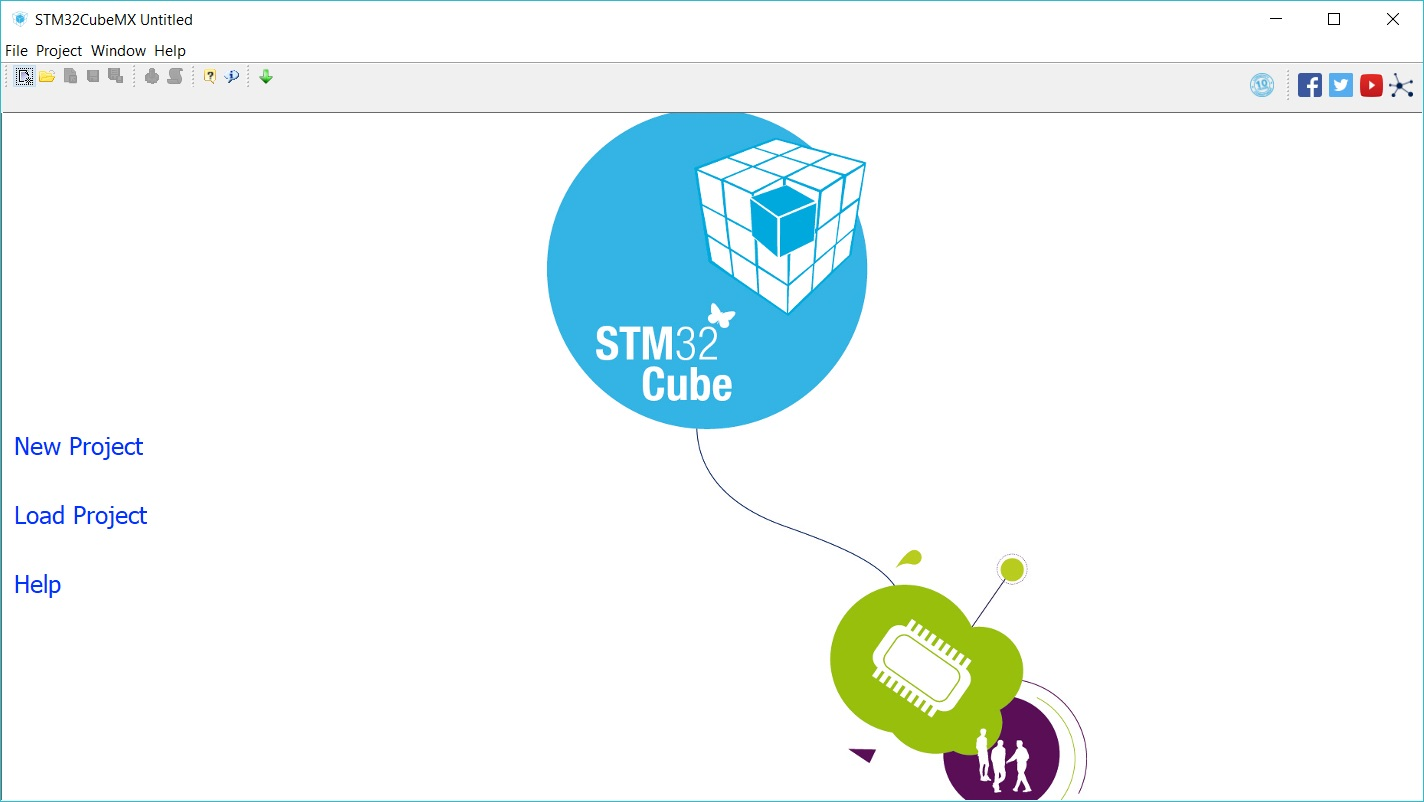
\includegraphics[width=11cm]{STM32CubeMX}
    \caption{Inicializador de proyectos STM32CubeMX}
    \label{fig:STM32CubeMX}
\end{figure}

La herramienta \textbf{STM32CubeMX} incluye una \textbf{base de datos de todos los microcontroladores disponibles}, permitiendo seleccionar el formato, encapsulado e incluso si se va a utilizar en su formato nucleo o en un kit de desarrollo. Incluye también documentación sobre cada microcontrolador y enlaces a distribuidores en caso de que el usuario final quiera comprarlo. 

\subsubsection{Asignación de funciones\label{sec:Configuracion_micro_asignacion}}

Tras seleccionar el microcontrolador, se presenta al usuario una \textbf{zona de trabajo dividida en cuatro pestañas}, cada una destinada a configurar un conjunto de características del microcontrolador: \textbf{pines y sus funciones, reloj, interfaces de comunicación y consumo de energía}.

\begin{figure} [h]
    \centering
    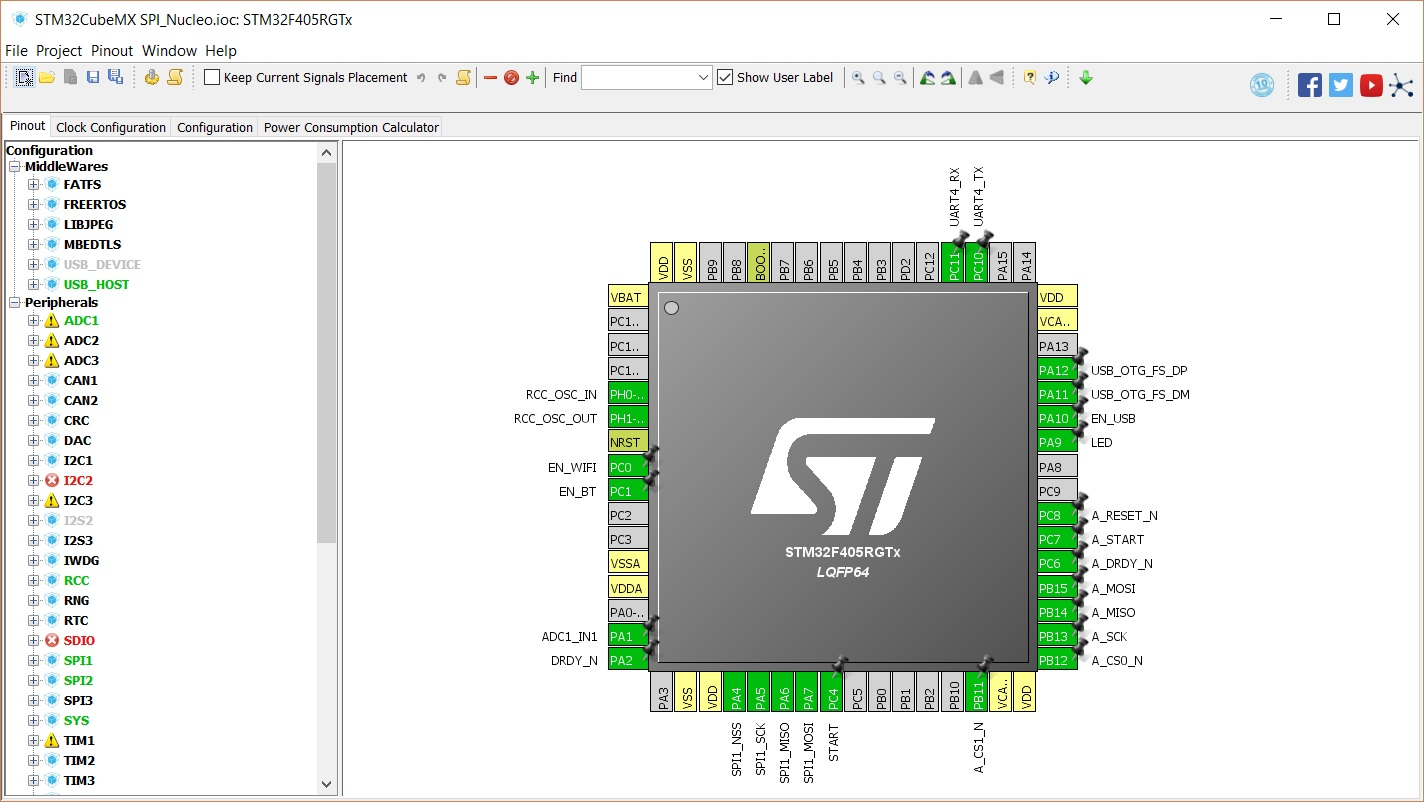
\includegraphics[width=15cm]{STM32CubeMX_pin}
    \caption{Espacio de trabajo del STM32CubeMX}
    \label{fig:STM32CubeMX_pin}
\end{figure}

La configuración de pines permite, no sólo ver de forma visual cada una de las funciones alternativas de cada pin, sino que además indica si alguna no está disponible y las alternativas en caso de existir.

\textbf{En la figura \ref{fig:STM32CubeMX_pin} aparece la configuración utilizada en este proyecto}. En la imagen se puede apreciar que todas las interfaces necesarias ya han sido asociadas a su pin correspondiente y aún quedan libres casi la mitad de los pines del total disponible. Esto es un indicador de la versatilidad de este dispositivo.

\subsubsection{Configuración de los relojes\label{sec:Configuracion_micro_reloj}}

En este apartado se explicará la configuración de los relojes del sistema. Se trata de un punto muy importante puesto que un reloj mal configurado puede provocar errores en la comunicación, una mala gestión del tiempo e incluso que el propio microcontrolador no arranque.

La interfaz desarrollada por STM muestra de forma visual todos los relojes que intervienen en el dispositivo así como las relaciones que hay entre ellos. De esta forma basta con seguir las líneas que conectan los distintos tipos de reloj para saber las dependencias que existen y los resultados que obtendrán en función de los valores escogidos.
\\En caso de que alguna configuración sea incorrecta la propia herramienta está preparada para ofrecer una solución que se acerque lo máximo posible a los resultados deseados.

\begin{figure} [h]
    \centering
    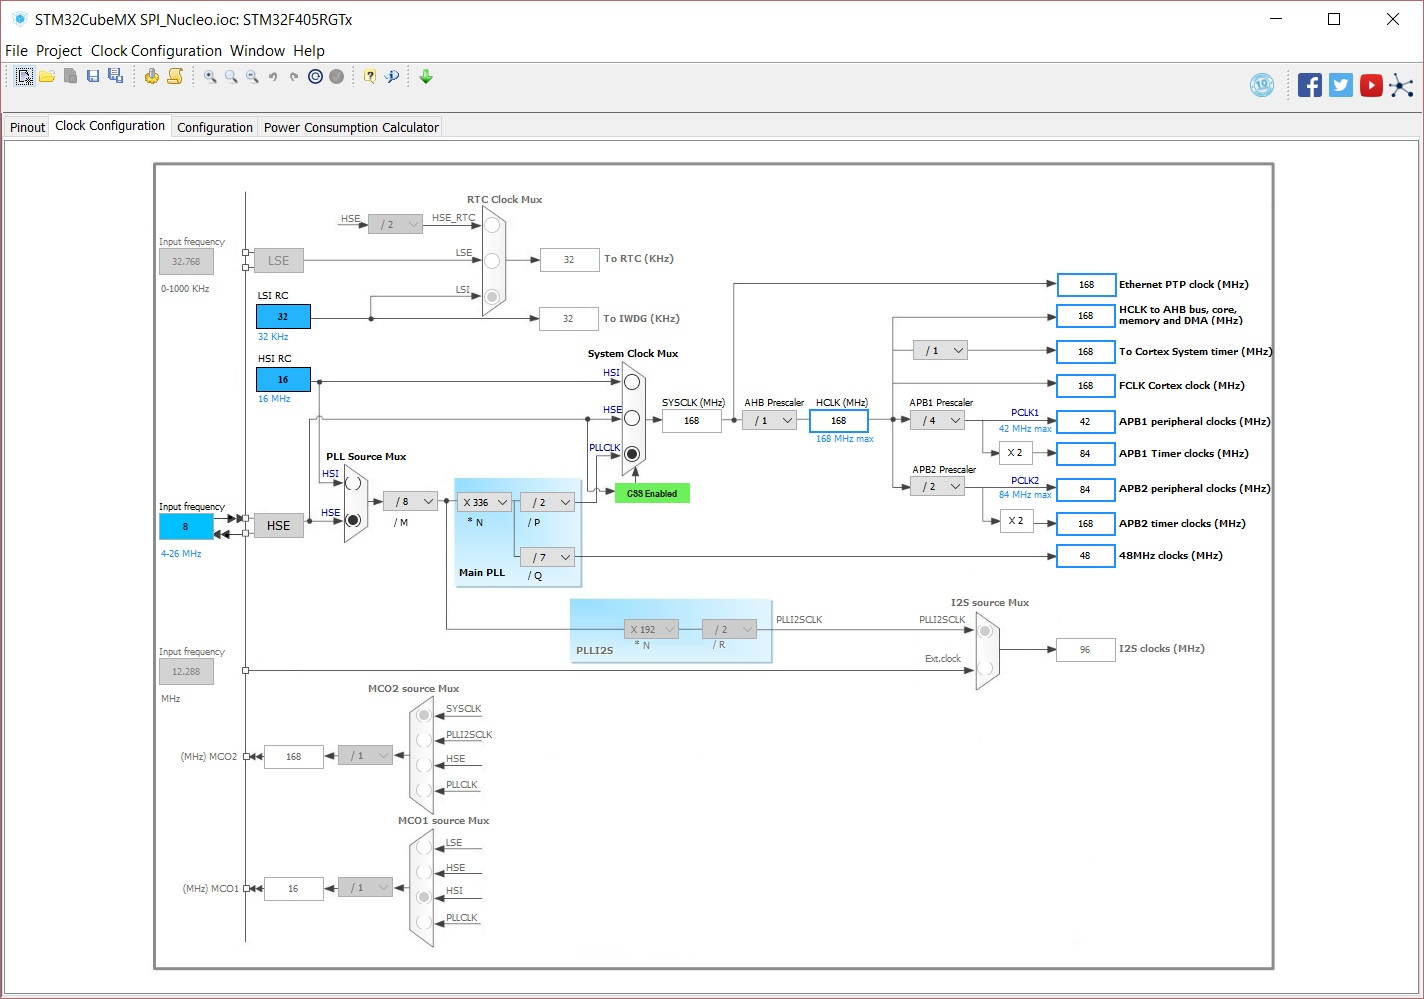
\includegraphics[width=16cm]{STM32CubeMX_clock}
    \caption{Configuración del reloj del microcontrolador}
    \label{fig:STM32CubeMX_clock}
\end{figure}

En \textbf{la figura \ref{fig:STM32CubeMX_clock} representa la configuración aplicada al microcontrolador} durante la realización de este proyecto. A la izquierda se muestran distintas fuentes disponibles mientras que a la derecha se ve la frecuencia final de reloj resultante en cada una de las partes del microcontrolador (periféricos, temporizadores, memoria, etc).

Como se puede ver, aprovecha ambos osciladores, el externo (\acrshort{HSE} = 8MHz) y el interno (\acrshort{LSI} = 16MHz) para, usando \acrshort{PLL}, generar un reloj de una frecuencia mucho más elevada (\textbf{168 MHz}). Dicha frecuencia es, según el fabricante, la \textbf{máxima frecuencia alcanzable por el dispositivo}.

La \textbf{función \acrshort{CSS}} garantiza que, en caso de fallo del reloj del microcontrolador, se genere una alerta y este entrare en modo seguro. Esta función es muy útil cuando se está trabajando con elementos en los que la seguridad de las personas depende directamente del correcto comportamiento microcontrolador.

\clearpage

\subsubsection{Configuración de los periféricos\label{sec:Configuracion_micro_com}}

La tercera pestaña permite \textbf{configurar los periféricos}, esto incluye interfaces de comunicación, puertos GPIO, USB, etc.

\begin{figure} [h]
    \centering
    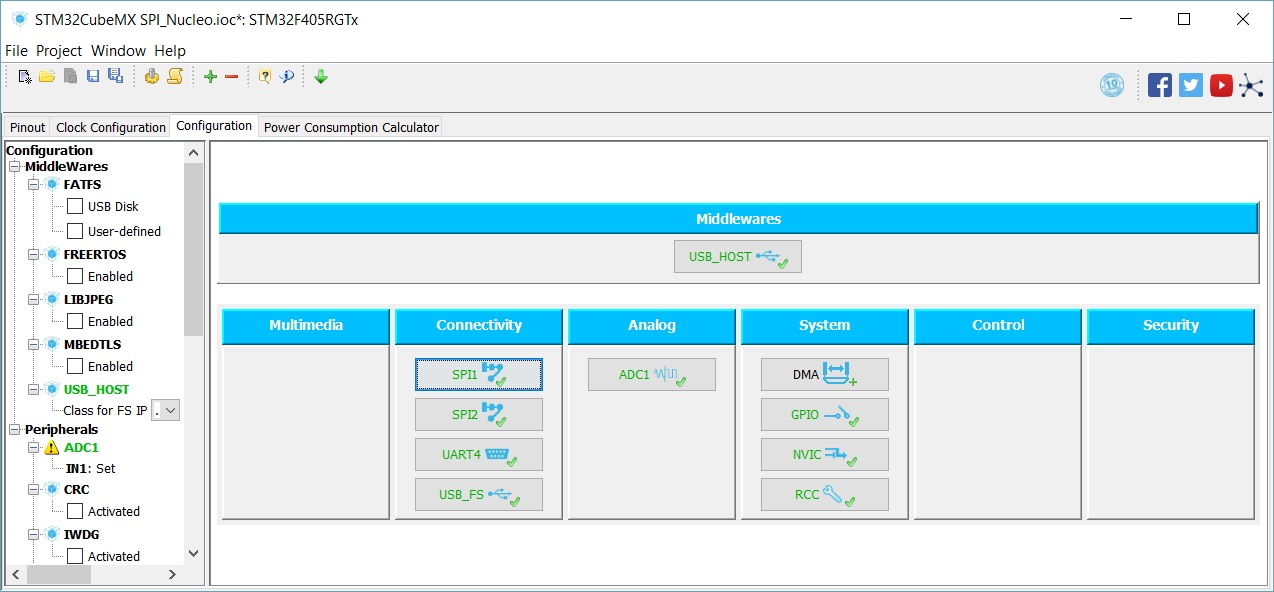
\includegraphics[width=15cm]{STM32CubeMX_conf}
    \caption{Configuración de las interfaces de comunicación}
    \label{fig:STM32CubeMX_conf}
\end{figure}

En función del estado del periférico este aparecerá marcado con un \textit{tick} verde indicando que todo está correctamente configurado o una cruz roja avisando que alguna característica podría no estar disponible. Además, será posible modificar la mayoría de las opciones relacionadas con ese periférico de forma intuitiva. 

\begin{figure} [h]
    \centering
    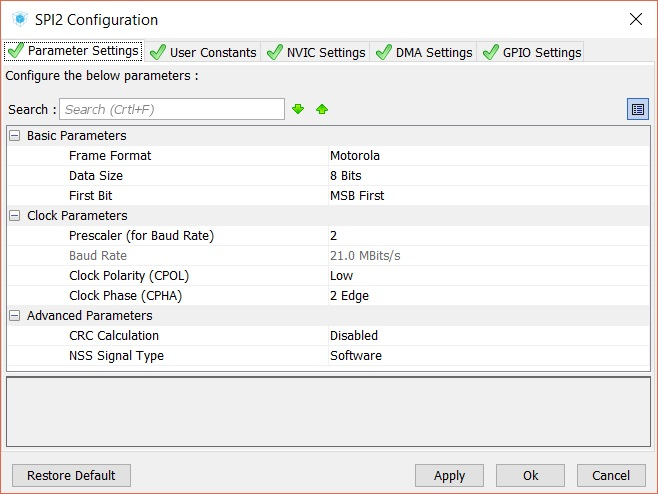
\includegraphics[width=10cm]{STM32CubeMX_conf_2}
    \caption{Detalle de la configuración de las interfaces de comunicación}
    \label{fig:STM32CubeMX_conf_2}
\end{figure}

En la figura \ref{fig:STM32CubeMX_conf_2} se muestran las opciones seleccionadas para el SPI que se comunicará con los ADS. Se puede cambiar la velocidad, el modo de transmisión e incluso si la gestión del pin $\overline{\text{CS}}$ se realizará de forma automática o manual.

\subsubsection{Cálculo de consumo\label{sec:Configuracion_micro_consumo}}

La última pestaña, ``\textit{Power Consuption Calculator}'', contiene numerosas opciones para el \textbf{análisis del consumo del microcontrolador}. En esta se puede estimar la \textbf{duración de la batería} en función de parámetros como el modo funcionamiento, el tipo de fuente de alimentación e incluso la temperatura.

\begin{figure} [h]
    \centering
    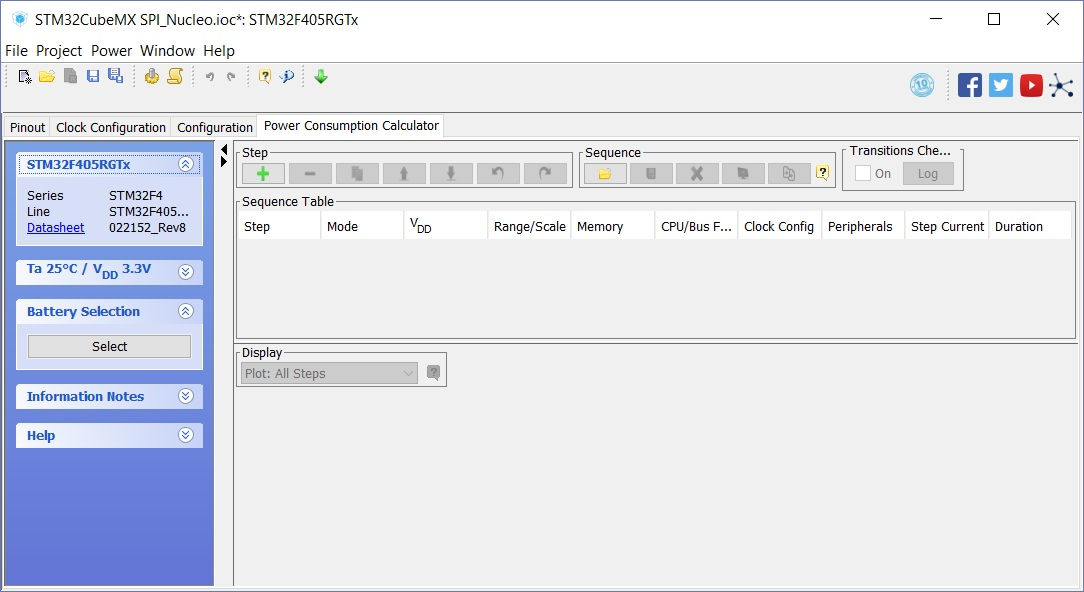
\includegraphics[width=15cm]{STM32CubeMX_otro}
    \caption{Calculadora del consumo del microcontrolador}
    \label{fig:STM32CubeMX_otro}
\end{figure}

\subsubsection{Generar código\label{sec:Configuracion_micro_generador}}

Finalmente se seleccionará el \textbf{\acrshort{IDE}} correspondiente para el cual el STM32CubeMX debe generar la base de código sobre la que se construirá el proyecto.

Esta herramienta es capaz de crear un código base para casi cualquier \acrshort{IDE}, pero de entre las opciones disponibles, \textbf{armKeil} es la herramienta que \textbf{presenta unos mejores resultados}. Dicho software crea el \textbf{código base} con la configuración seleccionada desde la interfaz y lo integra dentro de un proyecto ya configurado y listo para trabajar.

Es importante destacar que la utilización de STM32CubeMX no sólo está pensada para facilitar el comienzo del diseño proporcionando una base sobre la que trabajar, sino que también permite una \textbf{mayor portabilidad} del código ya que, si se siguen las reglas de programación sugeridas por la aplicación, esta permite realizar cambios de la configuración de los pines, los periféricos e incluso de familia de microcontrolador, todo ello \textbf{sin necesidad de reestructurar el código}.

\clearpage

El código que se ejecuta en el STM está dividido en \textbf{dos fases}. La primera, denominada comúnmente \textbf{\textit{setup}}, \textbf{sólo se ejecuta la primera vez} que se enciende el microcontrolador.
En esta se suelen declarar todas las variables globales, inicializar los periféricos y, en definitiva, preparar el microcontrolador para funcionar.

La segunda fase, denominada \textbf{\textit{loop}} es, como su nombre indica, un \textbf{bucle infinito}. En esta fase se ejecuta todo el código de forma cíclica. Normalmente en esta fase se incluye el funcionamiento normal del sistema, utilizando condicionales para forzar el comportamiento esperado.

Al generar el proyecto, el STM32CubeMX estructura el código tal como se muestra en el código \ref{algoritmo:Auto_gen}, dejando al usuario ciertas zonas libres para escribir en ellas y restringiendo la escritura en otras.

\begin{lstlisting}[label=algoritmo:Auto_gen,style = STM-code,frame=single,caption=Ejemplo de generación de código automáticamente]
  /* USER CODE BEGIN 1 */
	
  /* USER CODE END 1 */

  /* MCU Configuration----------------------------------------*/

  /* Reset of all peripherals, Initializes the Flash interface and the Systick. */
  HAL_Init();

  /* USER CODE BEGIN Init */

	
  /* USER CODE END Init */
\end{lstlisting}

Respetar dichas restricciones es opcional aunque una vez modificadas no se podrá cambiar a la configuración original del microcotrolador usando STM32CubeMX, pues dicha herramienta las utiliza como referencia y no respetarlas puede ocasionar la pérdida del trabajo.

Por simplicidad, comodidad y compatibilidad, durante la realización de este trabajo \textbf{se han respetado dichas restricciones} construyendo todo el código en las zonas habilitadas para ello.

\clearpage

\subsection{Implementación del firmware \label{sec:Software_micro_HAL}}

A lo largo de las siguientes páginas se presentará una introducción a los elementos software utilizados, haciendo especial hincapié en aquel código cuya función es indispensable para cumplir con las especificaciones fijadas al comienzo del proyecto.

\subsubsection{HAL \label{sec:Software_micro_HAL}}

La programación de microcontroladores basados en Arduino y su \acrshort{IDE} resulta especialmente intuitiva ya que desde sus comienzos ese era uno de los objetivos: acercar el mundo analógico y digital a gente poco versada en ello.

Los \textbf{ARM} de \textbf{STM} en cambio, están destinados a personas con cierta \textbf{experiencia programando microcontroladores}. Permiten libertad total proporcionando acceso a los registros sin restricciones y un control del hardware muy preciso. Si bien esta aproximación aumenta las posibilidades de la plataforma, también limita al número de personas que pueden ponerse a programar en ella así como la portabilidad de código.
\\Cuanto más cercano sea al hardware mayor exclusivo será y, por lo tanto, se requerirán más cambios para portar dicho código a otra familia si en el futuro las especificaciones varían o se desean mejorar las características del sistema.

Con esta problemática en mente los desarrolladores de STM crearon un conjunto de herramientas y drivers que reciben el nombre de \textbf{Hardware Abstraction Layer (\acrshort{HAL})}.

\begin{figure} [h]
    \centering
    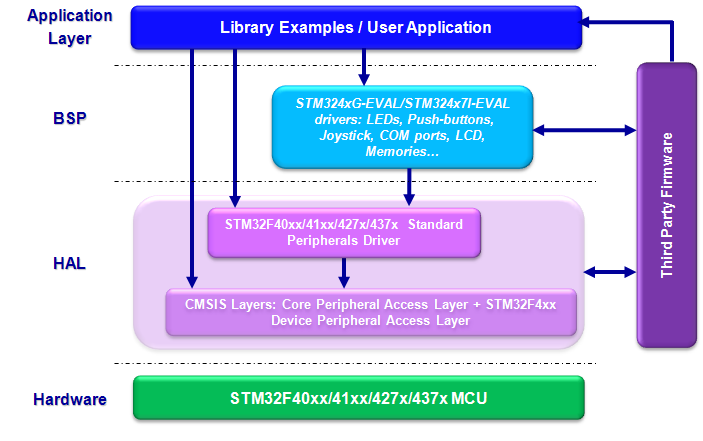
\includegraphics[width=13cm]{HAL-LL}
    \caption{Resumen del funcionamiento y características del HAL \cite{HAL-LL}}
    \label{fig:HAL-LL}
\end{figure}

La utilización de \acrshort{HAL} permite tanto portar código entre familias de STM como simplificar sensiblemente el desarrollo de un proyecto, pues integra un gran número de funciones relacionadas con la gestión de los distintos puertos de comunicaciones y GPIO así como otras encargadas de realizar \textbf{operaciones matemáticas complejas}.

\subsubsection{Estructura del código\label{sec:Software_micro_estados}}

El código está organizado siguiendo el esquema típico de una \textbf{máquina de estados}. Haciendo uso de condicionales de tipo ``switch - case'' se ha construído el programa representado en la figura \ref{fig:Maquina_estados_STM}. 

\begin{figure} [h]
    \centering
    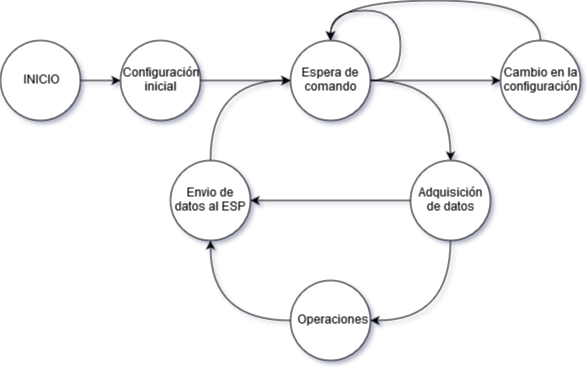
\includegraphics[width=14cm]{Maquina_estados_STM}
    \caption{Estructura del programa}
    \label{fig:Maquina_estados_STM}
\end{figure}

\textbf{En primer lugar} se realiza una \textbf{inicialización} de todas las variables, los periféricos y el resto de dispositivos que se encuentran conectados con el STM.

A continuación, el \textbf{microcontrolador} se queda \textbf{a la espera de un comando por parte del ESP-12E} que le indicará que hacer. Por el momento se han implementado \textbf{tres alternativas}, dos relacionadas con la adquisición de datos y una para cambios de   configuración, pero está preparado para aumentar el número de condiciones con facilidad. De esta forma el software puede aumentar en funcionalidades sin que haya que reestructurar el código.

Si el microcontrolador recibe la orden de \textbf{adquirir datos}, este activa la comunicación SPI y queda a la espera de una confirmación por parte del ADS de que los datos están listos para ser leídos del bus.

Tras leer los datos el microcontrolador convierte la información a formato \textit{float} y calcula la equivalencia en voltaje de la medida. 

Posteriormente, en función de la orden recibida desde el ESP, el STM \textbf{transmite la información al ESP} o bien \textbf{realiza operaciones matemáticas sobre los datos} y finalmente los transmite al ESP. Estas operaciones pueden ser sumas, restas e incluso un filtrado de la señal para eliminar componentes indeseadas.

\subsubsection{Transmisión de datos por SPI \label{sec:Software_micro_SPI}}

Aunque la capa de abstracción del hardware facilita notablemente el trabajo de desarrollo, para poder trabajar con un bus de comunicaciones de forma eficiente y sin errores es necesario saber como funciona a nivel hardware y, desde ahí, realizar una abstracción progresiva. 

En primer lugar será importante definir que elemento hará las \textbf{funciones de Máster y cual de Esclavo}, pues esto limitará las características de la comunicación y forzará la configuración de los \acrshort{GPIO} de una forma u otra.

\begin{figure} [h]
    \centering
    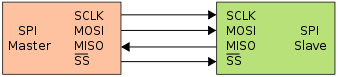
\includegraphics[width=10cm]{SPI_Master_Slave}
    \caption{Esquema de comunicaciones SPI \cite{wikipedia}}
    \label{fig:SPI_Master_Slave}
\end{figure}

Para aprovechar la tasa de transferencia del SPI del STM al máximo lo ideal sería que fuese este el Máster en ambas comunicaciones (hacia el ADS y hacia el ESP). Esto es así porque la máxima velocidad de transmisión es definida por el Máster mientras que el Esclavo se adapta a las normas impuestas, siempre dentro de unos rangos establecidos por el fabricante.

Por desgracia, las limitaciones de las librerías disponibles para el \textbf{ESP-12E} fuerzan que este sea obligatoriamente el \textbf{Máster} de esa comunicación limitando la velocidad a la máxima que sea capaz de alcanzar el ESP.

Para la \textbf{transmisión de datos desde el STM} es muy importante tener en cuenta que el microcontrolador trabaja a bajo nivel. Las funciones implementadas en los \textit{drivers} y librerías de abstracción de hardware facilitan el trabajo, pero debe tenerse presente en todo momento que se está transmitiendo información de registros de memoria y, por lo tanto, no se debe perder de vista el \textbf{tamaño} del dato ni el \textbf{tipo} del mismo.

Las funciones encargadas de transmitir información a través del puerto \textbf{\acrshort{SPI}} son:
\begin{itemize}
\item HAL\_StatusTypeDef HAL\_SPI\_Transmit
\item HAL\_StatusTypeDef HAL\_SPI\_Receive
\item HAL\_StatusTypeDef HAL\_SPI\_TransmitReceive
\end{itemize}

Las tres funciones necesitan el puntero al puerto por el que se transmitirá la información, la dirección de memoria de la misma, el tamaño del conjunto de datos y el tiempo de espera por cada transmisión.

El código \ref{algoritmo:STM_Transmision_SPI} muestra la \textbf{cabecera de la función} encargada de \textbf{transmitir y recibir información} de forma simultánea. En él se puede ver con claridad el tipo de datos que necesita para realizar una transmisión satisfactoria.

\begin{lstlisting}[label=algoritmo:STM_Transmision_SPI,style = STM-code,frame=single,caption=Transmisión de datos a través de SPI con el STM]
HAL_StatusTypeDef HAL_SPI_TransmitReceive(
	SPI_HandleTypeDef *hspi,
 	uint8_t *pTxData, 
 	uint8_t *pRxData, 
 	uint16_t Size, 
	uint32_t Timeout)
\end{lstlisting}

Las funciones encargadas de transmitir y recibir información, ya sea a través de \acrshort{SPI} o a través de otro periférico, actúan de forma similar y necesitan las mismas variables. A pesar de que la función simplifica sensiblemente la gestión de memoria y pines, aún es necesario tener en cuenta ciertas limitaciones que marcarán el modo de trabajo:
\begin{itemize}
\item \textbf{Tamaño de transmisión fijo}\\
El tamaño de los datos a transmitir debe ser de 8 bits. En caso de querer transmitir una variable cuyo tamaño en memoria sea superior será necesario realizar una transformación.
\item \textbf{Gestión de pines manual o automática}\\
La gestión de pines como ``$\overline{\text{DRDY}}$'' y ``\textsc{Start}'' se debe realizar de forma manual. ``$\overline{\text{CS}}$'', en cambio, está pensado para ser gestionado de forma manual o automática en función de las circunstancias.
\item \textbf{Gestión de memoria}\\
El STM es capaz de transmitir una gran cantidad de datos por \acrshort{SPI}. Es importante tener claro la cantidad de datos a recibir o transmitir, pues equivocarse puede suponer acceder a una dirección de memoria no permitida, recibir valores incorrectos o incluso corromper el código y forzar el reinicio del microcontrolador.
\end{itemize}

Al ser obligatorio transmitir datos de 8bits se vuelve indispensable crear algún metodo para poder dividir aquellas variables cuyos tamaño sea superior (float, long, etc).
El tipo de dato \textbf{union} definido en \textbf{C} está pensado justo para este cometido. Permite definir varias variables cuyo tamaño total sea equivalente y asignar la misma dirección de memoria a todas ellas. A continuación se muestra un fragmento del código necesario para dividir una variable \textbf{long} (32bits) en un array de 4 posiciones de tipo \textbf{int} (8bits cada una).

\begin{lstlisting}[label=algoritmo:STM_Divisor,style = STM-code,frame=single,caption=División de variables en otras de menor tamaño]
union miDato{
	struct
	{
		uint8_t  b[4];     // Array de bytes de tamaño equivalente
	}split;
		long dato;
} long_data; 
\end{lstlisting}
\clearpage

\subsubsection{Comunicación con el ADS \label{sec:Software_micro_ADS}}

El \textbf{ADS} está preparado para recibir y transmitir información a través del puerto SPI integrado. Aunque puede transmitir información, el integrado sólo es capaz de actuar en \textbf{modo Esclavo} y \textbf{\textit{\gls{Full Duplex}}}.

La memoria del ADS está organizada en distintos registros, cada uno de los cuales tiene una función definida en la hoja de características del componente. La \textbf{configuración} del dispositivo se realiza de forma casi exclusiva mediante SPI \textbf{escribiendo directamente sobre el registro deseado}.

Al tratarse de registros de memoria, para su modificación resulta indispensable conocer su posición exacta. Aunque para una máquina esto no es un problema, para un ser humano puede resultar complicado recordar e identificar de forma eficiente cada uno de ellos. 
\\Para que la asociación sea más sencilla se ha creado un archivo ``.h'' con definiciones de todos los registros, asociando cada uno de ellos a un comando. Un ejemplo que ilustra esta problemática sería la modificación de los GPIO del ADS. Para poder realizar esta acción sin asociaciones sería necesario conocer que la dirección de memoria asociada al GPIO es la 0x14 mientras que tras la asociación basta con escribir en el registro \textsc{GPIO} y el microcontrolador se encargará de traducir este símbolo a su valor correspondiente. Con esta transformación se consigue además \textbf{aumentar la legibilidad del código}.

\begin{lstlisting}[label=algoritmo:STM_ADS_def,style = STM-code,frame=single,caption=Ejemplo de definiciones de los registros y funciones del ADS]
//Position in memory of registers: (Pg. 39)

#define ID 						0x00	// (0000 0000)
#define CONFIG1  		 	0x01	// (0000 0001) 
#define CONFIG2  			0x02 	// (0000 0010)
.		.						  .					.
#define CONFIG4   		0x17 	// (0001 0111)
\end{lstlisting}

El manual de funcionamiento del ADS muestra distintas formas de configuración. Es posible \textbf{leer y/o escribir un registro} o varios de forma simultánea con pocos comandos. De acuerdo al manual, para realizar una escritura de un registro es necesario transmitir \textbf{tres datos al ADS}. El primero indicará la \textbf{dirección de memoria} sobre la que se trabajará. El segundo sirve para seleccionar el \textbf{número de registros} a escribir. Por último el tercer dato es el que se almacenará en memoria.

\begin{figure} [H]
    \centering
    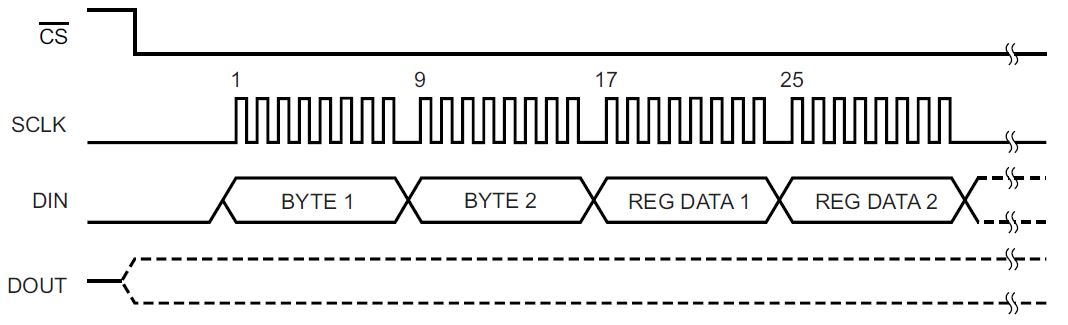
\includegraphics[width=13cm]{ADS_wreg}
    \caption{Escritura de dos registros del ADS \cite{Datasheet_ADS}}
    \label{fig:ADS_wreg}
\end{figure}

El código generado en el STM para realizar esta función es el presentado en \ref{algoritmo:STM_wreg}.

\begin{lstlisting}[label=algoritmo:STM_wreg,style = STM-code,frame=single,caption=Escritura en registros del ADS]
void adc_wreg(uint8_t reg, uint8_t val, SPI_HandleTypeDef *SPI){
	uint8_t zero_t = 0x00;
	uint8_t zero_r = 0x00;
	uint8_t reg_temp = WREG | reg;
	uint8_t val_temp = val;
	
	HAL_GPIO_WritePin(A_CS0_N_GPIO_Port, A_CS0_N_Pin, GPIO_PIN_RESET);
	HAL_SPI_TransmitReceive(SPI, &reg_temp, &zero_r, 1, 100);
	HAL_SPI_TransmitReceive(SPI, &zero_t, &zero_r, 1, 100);	
	HAL_SPI_TransmitReceive(SPI, &val_temp, &zero_r, 1, 100);	

	HAL_Delay(1);
	HAL_GPIO_WritePin(A_CS0_N_GPIO_Port, A_CS0_N_Pin, GPIO_PIN_SET);
}
\end{lstlisting}

La \textbf{lectura de los registros del ADS} se realiza de una forma análoga. En esta ocasión se transmiten los mismos dos datos que para escribir en un registro siendo la única diferencia que el tercer dato (y los siguientes en caso de ser más de un registro) se transmitirán desde el ADS hacia el STM tal y como aparece en la figura \ref{fig:ADS_rreg}.

\begin{figure} [h]
    \centering
    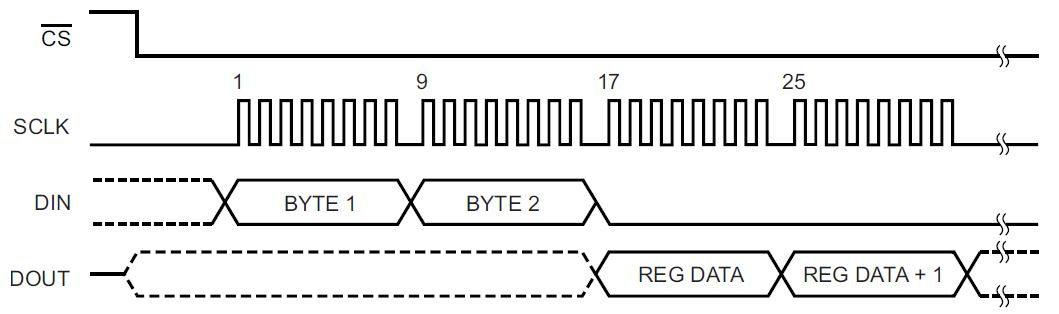
\includegraphics[width=13cm]{ADS_rreg}
    \caption{Lectura de dos registros del ADS \cite{Datasheet_ADS}}
    \label{fig:ADS_rreg}
\end{figure}

\begin{lstlisting}[label=algoritmo:STM_rreg,style = STM-code,frame=single,caption=Lectura de registros del ADS]
uint8_t adc_rreg(uint8_t reg, SPI_HandleTypeDef *SPI){
	uint8_t val = 0x00;
	uint8_t zero_t = 0x00;
	uint8_t zero_r = 0x00;
	uint8_t temp = RREG | reg;
	
	HAL_GPIO_WritePin(A_CS0_N_GPIO_Port, A_CS0_N_Pin, GPIO_PIN_RESET);
	HAL_SPI_TransmitReceive(SPI, &temp, &zero_r, 1, 100);
	HAL_SPI_TransmitReceive(SPI, &zero_t, &zero_r, 1, 100);	
	HAL_SPI_TransmitReceive(SPI, &zero_t, &val, 1, 100);

	HAL_Delay(1);
	HAL_GPIO_WritePin(A_CS0_N_GPIO_Port, A_CS0_N_Pin, GPIO_PIN_SET);

	return val;
}
\end{lstlisting}

Para que la transmisión sea correcta es muy importante que todas las variables definidas sean independientes. Además, el ADS necesita que durante la lectura de datos el pin \textsc{MOSI} se mantenga en un 0 lógico todo el rato.

\subsubsection{Lectura y conversión de datos \label{sec:Software_micro_Datos}}

El ADS está construído utilizando un sistema adquisidor de 8 canales, todos adquiridos de forma simultánea utilizando un sistema $\Delta\Sigma$ de 24 bits y ganancia variable.

Tras adquirir los datos estos son codificados siguiendo el siguiente formato:
\begin{table} [H]
 \centering
 \begin{tabular}{|c|c|}
 \hline 
\textbf{Señal de entrada, V$_{IN}$} &  \multirow{2}{*}{\textbf{Código de salida ideal}}\\ 
 \textbf{(INxP - INxN)} &  \\ 
 \hline 
 +FS & 7FFFFFh\\ 
 \hline 
 +FS$/(2^{23}-1)$ & 000001h \\ 
 \hline 
 0 & 000000h\\ 
 \hline 
 -FS & FFFFFFh\\ 
 \hline 
 +FS$(2^{23}/(2^{23}-1))$ & 800000 \\ 
 \hline 
 \end{tabular} 
 \caption{Equivalencia de voltaje ideal de entrada y código de salida}
 \label{tab:ADS_equivalencia}
\end{table}

La tabla anterior es una modificación de la proporcionada en la hoja de características del ADS corrigiendo algunas pequeñas erratas. La variable ``FS'' corresponde a la escala completa de entrada del ADS. En este caso son 4.5V divididos por la ganancia (G).

Para \textbf{voltajes positivos} la decodificación de estos valores es muy sencilla, pues basta con aplicar una simple \textbf{regla de tres} en la que cada bit es un incremento de $4.5V/(2^{23}*G)$.\\
Para \textbf{voltajes negativos} basta con \textbf{invertir} todos los bits y aplicar la misma regla de tres.\\
El bit más significativo indica si el voltaje final será positivo (0) o negativo (1) y es el que se ha usado como referencia para aplicar la conversión anterior en caso de ser necesaria.

Al trabajar con datos de 24 bits no es posible realizar una inversión directa del valor de la variable o los 8 bits más significativos se verían invertidos también. Por suerte el ADS transmite los datos en paquetes de 8 bits lo cual facilita tratarlos de forma independiente y, tras hacer la transformación a nivel de bit, crear una variable que represente el valor real.

Unir los tres bytes una vez se ha realizado la conversión es posible de múltiples formas. Por motivos de eficiencia y de reutilización del código se ha realizado la misma aproximación ya expuesta previamente haciendo uso de datos de tipo \textbf{union}.

El código \ref{algoritmo:ADS_decodificacion}, incluído en una librería creada para interactuar con el ADS, es el utilizado para este fin.

\clearpage

\begin{lstlisting}[label=algoritmo:ADS_decodificacion,style = STM-code,frame=single,caption=Decodificación de datos binarios a Voltajes]
float32_t byte2float (uint8_t data_23_16, uint8_t data_15_8, uint8_t data_7_0, uint8_t ganancia)
	{
		float32_t value = 0;
		
		union miDato{
		struct
		{
			uint8_t  b[4];     // Array de bytes de tamaño igual al tamaño de la primera variable: int = 2 bytes, float = 4 bytes
		}split;
			long dato;
	 } long_data; 
		
	 long_data.dato = 0;
	 
		if (data_23_16>=0x80) //1000 0000
		{
			long_data.split.b[2] = ~data_23_16;
			long_data.split.b[1] = ~data_15_8;
			long_data.split.b[0] = ~data_7_0;
			value = long_data.dato;
			value = -value;
		}
		else
		{
			long_data.split.b[2] = data_23_16;
			long_data.split.b[1] = data_15_8;
			long_data.split.b[0] = data_7_0;
			value = long_data.dato;
		}
		
		value = value*4.5f/(8388607.0f*ganancia); //4.5/(2^23*G)
		
		return value;
	}
\end{lstlisting}

El código anterior realiza una conversión triple: 4 bytes $\Rightarrow$ long $\Rightarrow$ float, donde el valor final devuelto es el voltaje real medido una vez se ha aplicado el factor de ganancia correspondiente.

El ADS tiene embebido un sistema de control basado en comandos a través de SPI. Estos comandos permiten realizar ciertas operaciones en tiempo real que facilitan el control del integrado y amplian sus características. 

La tabla \ref{tab:ADS_comandos}, sacada de la hoja de características del componente, muestra todos los comandos que el ADS es capaz de reconocer, sus funciones y el conjunto de bytes que representa cada uno. Los últimos dos comandos corresponden a la lectura y escritura en registros y ya han sido explicados previamente.

\begin{table}[H]
    \centering
    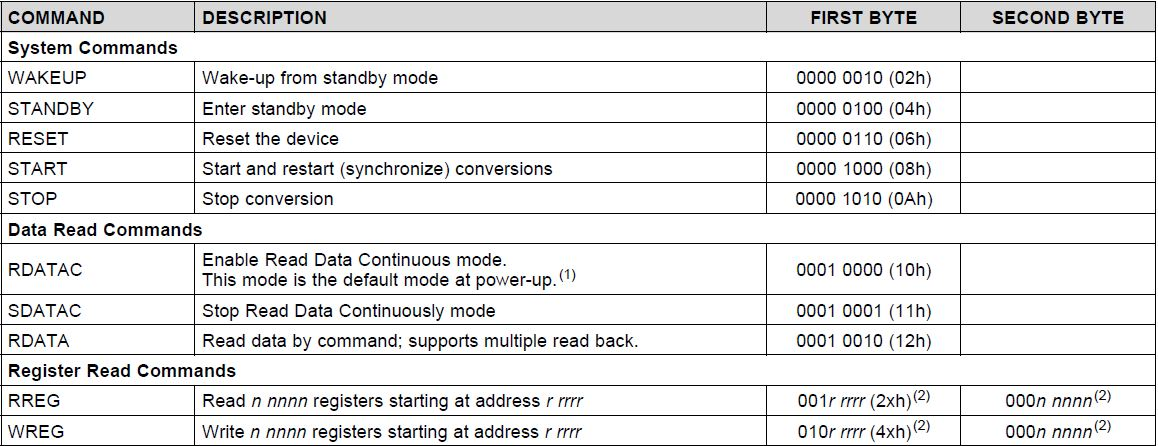
\includegraphics[width=16cm]{ADS_comandos}
    \caption{Comandos del ADS1299}
    \label{tab:ADS_comandos}
\end{table}

Durante la realización de este proyecto ha sido necesario utilizar la mayor parte de los comandos presentados en la tabla anterior. Cabe destacar que aquellos categorizados como ``Comandos del sistema'' han sido necesarios durante la secuencia de inicio del ADS casi en exclusiva, pues no se han implementado funciones de ahorro de energía. Estas se han contemplado como una mejora a llevar a cabo en futuras iteraciones de este proyecto.

El ADS cuenta con dos modos de lectura: continua y bajo demanda. Los comandos categorizados como ``Comandos de lectura'' están relacionados con la gestión de estos dos modos y se dividen a su vez en dos tipos según su función:
\begin{itemize}
\item \textbf{Configuración}\\
\textsc{RDATAC} y \textsc{SDATAC} activan y desactivan el modo de lectura continua respectivamente. El ADS se encuentra por defecto en modo continuo tras completar la secuencia de inicio.
\item \textbf{Lectura}\\
\textsc{RDATA} solicita en el modo de lectura bajo demanda la transmisión de los datos capturados en ese momento.
\end{itemize} 

El modo bajo demanda está pensado para aquellos sistemas en los que es necesario adquirir poca información a lo largo del tiempo. En esta configuración el ADS se mantiene inactivo hasta que recibe el comando de lectura y sólo entonces es cuando la realiza. Este comportamiento favorece la implementación de sistemas de ahorro de energía basados en los comandos \textsc{STANDBY} y \textsc{WAKEUP}. De esta forma es posible aumentar la autonomía del sistema completo considerablemente.

Por desgracia, este modo no es compatible con la transmisión de grandes cantidades de datos o mediciones muy continuas. Por cada medida es necesario utilizar el comando \textsc{RDATA}, afectando directamente al rendimiento y eficiencia en la transmisión.

La figura \ref{fig:ADS_SDATAC} ilustra la transmisión de información usando el modo bajo demanda.

\begin{figure} [H]
    \centering
    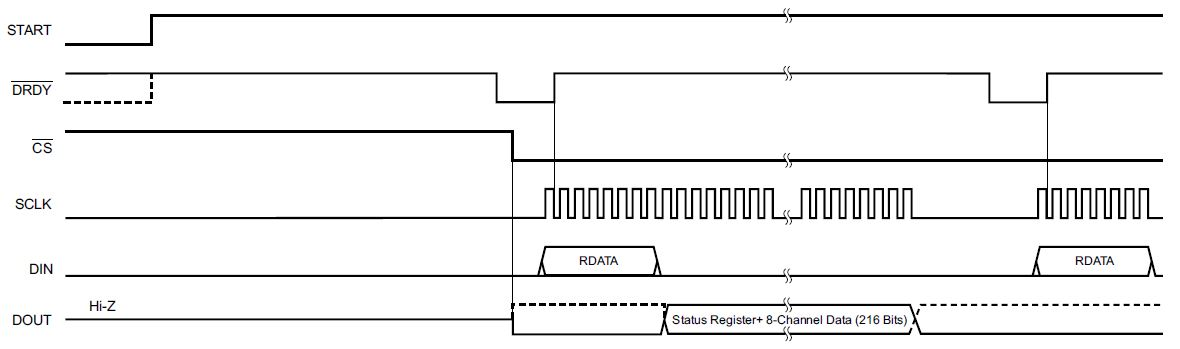
\includegraphics[width=15cm]{ADS_SDATAC}
    \caption{Modo de uso del comando \textsc{RDATA}}
    \label{fig:ADS_SDATAC}
\end{figure}

Por los motivos explicados anteriormente este modo no será utilizado normalmente pero aún así se ha decidido trabajar en su implementación en caso de que fuese necesario en el futuro. El código utilizado para adquirir datos es el siguiente:

\begin{lstlisting}[label=algoritmo:ADS_oneshot,style = STM-code,frame=single,caption=Lectura de datos en modo \textit{one-shot}]
void one_shot (uint8_t data[], SPI_HandleTypeDef *SPI)
{
	uint8_t zero = 0x00;
	uint8_t cmd = RDATA;
			
	while (HAL_GPIO_ReadPin(A_DRDY_N_GPIO_Port, A_DRDY_N_Pin) == GPIO_PIN_SET){}

	HAL_GPIO_WritePin(A_CS0_N_GPIO_Port, A_CS0_N_Pin, GPIO_PIN_RESET);
	
	HAL_SPI_TransmitReceive(SPI, &cmd, &zero,  1, 100);

	read_data_frame(data, SPI);
			
	while (HAL_GPIO_ReadPin(A_DRDY_N_GPIO_Port, A_DRDY_N_Pin) == GPIO_PIN_RESET) {}			
				
	HAL_GPIO_WritePin(A_CS0_N_GPIO_Port, A_CS0_N_Pin, GPIO_PIN_SET);

	update_bias_ref(data, SPI);
}
\end{lstlisting}

Para recibir una gran cantidad de información de forma ininterrumpida el ADS cuenta con el modo continuo. Se transmite el comando \textsc{RDATAC} y desde ese momento el ADS empieza a adquirir información y transmitirla. El pin $\overline{\text{DRDY}}$ es utilizado por el ADS para indicar que la siguiente tanda de datos está disponible para su lectura. 

La figura \ref{fig:ADS_RDATAC} representa la transmisión de información en modo continuo y el código \ref{algoritmo:ADS_continuo} el código equivalente.

\begin{figure} [H]
    \centering
    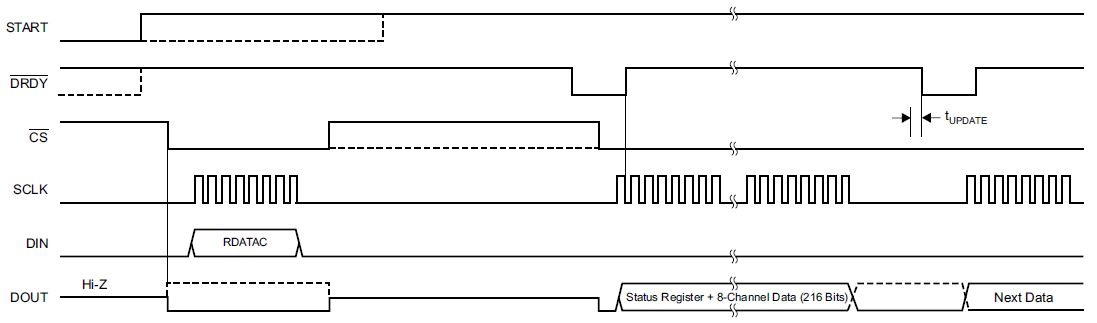
\includegraphics[width=16cm]{ADS_RDATAC}
    \caption{Transmisión de datos en modo continuo}
    \label{fig:ADS_RDATAC}
\end{figure}

\begin{lstlisting}[label=algoritmo:ADS_continuo,style = STM-code,frame=single,caption=Lectura de datos en modo continuo]
void adquire_array_data (uint8_t data[], float32_t channel_1[],float32_t channel_2[],float32_t channel_3[],float32_t channel_4[],float32_t channel_5[],float32_t channel_6[],float32_t channel_7[],float32_t channel_8[], uint8_t gain[], SPI_HandleTypeDef *SPI)
{
	int debug = 255;
	// read LENGTH_SAMPLES samples
		
	adc_send_command(RDATAC, SPI);
		
	while (HAL_GPIO_ReadPin(A_DRDY_N_GPIO_Port, A_DRDY_N_Pin) == GPIO_PIN_SET){}
		
	HAL_GPIO_WritePin(A_CS0_N_GPIO_Port, A_CS0_N_Pin, GPIO_PIN_RESET);
		
	read_data_frame(data, SPI);
			
	channel_1[0]=byte2float(data[1*3], data[1*3+1], data[1*3+2], gain[0]);
	channel_2[0]=byte2float(data[2*3], data[2*3+1], data[2*3+2], gain[1]);
	channel_3[0]=byte2float(data[3*3], data[3*3+1], data[3*3+2], gain[2]);
	channel_4[0]=byte2float(data[4*3], data[4*3+1], data[4*3+2], gain[3]);
	channel_5[0]=byte2float(data[5*3], data[5*3+1], data[5*3+2], gain[4]);
	channel_6[0]=byte2float(data[6*3], data[6*3+1], data[6*3+2], gain[5]);
	channel_7[0]=byte2float(data[7*3], data[7*3+1], data[7*3+2], gain[6]);
	channel_8[0]=byte2float(data[8*3], data[8*3+1], data[8*3+2], gain[7]);
			
	while (HAL_GPIO_ReadPin(A_DRDY_N_GPIO_Port, A_DRDY_N_Pin) == GPIO_PIN_RESET){}
			
	for (int i = 1; i<LENGTH_SAMPLES; i++)
	{
		while (HAL_GPIO_ReadPin(A_DRDY_N_GPIO_Port, A_DRDY_N_Pin) == GPIO_PIN_SET){}
			
		read_data_frame(data, SPI);

		channel_1[i]=byte2float(data[1*3], data[1*3+1], data[1*3+2], gain[0]);
		channel_2[i]=byte2float(data[2*3], data[2*3+1], data[2*3+2], gain[1]);
		channel_3[i]=byte2float(data[3*3], data[3*3+1], data[3*3+2], gain[2]);
		channel_4[i]=byte2float(data[4*3], data[4*3+1], data[4*3+2], gain[3]);
		channel_5[i]=byte2float(data[5*3], data[5*3+1], data[5*3+2], gain[4]);
		channel_6[i]=byte2float(data[6*3], data[6*3+1], data[6*3+2], gain[5]);
		channel_7[i]=byte2float(data[7*3], data[7*3+1], data[7*3+2], gain[6]);
		channel_8[i]=byte2float(data[8*3], data[8*3+1], data[8*3+2], gain[7]);
				
		while (HAL_GPIO_ReadPin(A_DRDY_N_GPIO_Port, A_DRDY_N_Pin) == GPIO_PIN_RESET){}
	}
		
	HAL_GPIO_WritePin(A_CS0_N_GPIO_Port, A_CS0_N_Pin, GPIO_PIN_SET);
}
\end{lstlisting}

El STM no permite trabajar con vectores de varias dimensiones de la misma forma que otros lenguajes de programación, así que para capturar todos los canales ha sido necesario repetir código. A cambio, el escalado del código de un canal a varios se realiza de una forma sencilla e intuitiva. En posteriores revisiones de este proyecto se valorará su sustitución por otro sistema más eficiente.

\subsubsection{DSP - Implementación de filtros \label{sec:Software_micro_DSP}}

Una de las características que diferencian los microcontroladores de esta familia de los de otras es la capacidad de realizar operaciones matemáticas sin que ello repercuta de forma muy significativa en el rendimiento. 

Para facilitar su utilización y unificar a todos los desarrolladores ARM ha creado una librería llamada CMSIS-DSP que engloba todas las funcionalidades de procesado de señal más comunes, optimizando dichos algoritmos para hacerlos lo más eficientes posible.
Esta librería incluye los siguientes tipos de operaciones:

\begin{itemize}
\item Operaciones matemáticas básicas, rápidas y complejas
\item \textbf{Filtrado}
\item Matrices
\item Transformaciones
\item Estadísticas
\item Controladores (PID, senos, etc)
\item Interpolación
\item Apoyo
\end{itemize}

Estas funciones utilizan variables de tipo enteros de 8, 16 y 32 bits y float de 32 bits. En esta ocasión se han utilizado exclusivamente las funciones de filtrado de señal, concretamente aquellas dedicadas a la realización de filtros FIR y su aplicación a señales.

ARM ha puesto a disposición de los consumidores una página web de referencia en la que se puede encontrar una descripción detallada de cada función incluyendo su modo de uso y ejemplos \cite{CMSIS-DSP}.

El filtrado de una señal con un filtro FIR en ARM es un proceso sencillo pero que engloba varias herramientas, pues el diseño del filtro se debe realizar de forma independiente. La función utilizada para este fin es ``arm\_fir\_f32()''. \\
Esta función recibe una señal en formato \textbf{float32\_t} (x[n]), los coeficientes del filtro y la longitud de la ventana y devuelve una señal filtrada (y[n]) con las características deseadas.
\begin{figure} [h]
    \centering
    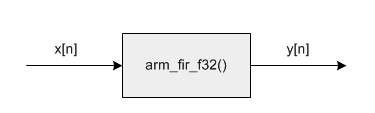
\includegraphics[width=7cm]{arm_fir_f32}
    \caption{Diagrama de bloques del filtrado de una señal x[n]}
    \label{fig:arm_fir_f32}
\end{figure}

El código necesario para aplicar un filtro FIR a una señal es el siguiente:

\begin{lstlisting}[label=algoritmo:STM_filtro,style = STM-code,frame=single,caption=Filtro FIR en STM]
/* ----------------------------------------------------------------------
** Includes necesarios
** ------------------------------------------------------------------- */
#include "arm_math.h"
#include "math_helper.h"
const float32_t firCoeffs32[NUM_TAPS] = {h1, h2, ....,hn}
/* ------------------------------------------------------------------
 * Variables globales para el filtro FIR
 * ------------------------------------------------------------------- */
uint32_t blockSize = BLOCK_SIZE;
uint32_t numBlocks = TEST_LENGTH_SAMPLES/BLOCK_SIZE;
 * ------------------------------------------------------------------- */
arm_fir_instance_f32 S;
arm_status status;
float32_t  *inputF32, *outputF32;
/* Inicialización de buffers de entrada y salida */
inputF32 = &testInput_f32_1kHz_15kHz[0];
outputF32 = &testOutput[0];
/* Inicialización de la estructura de la instancia del filtro FIR. */
arm_fir_init_f32(&S, NUM_TAPS, (float32_t *)&firCoeffs32[0], &firStateF32[0], blockSize);
/* ----------------------------------------------------------------------
** Aplicación del filtro a cada conjunto de blockSize
** ------------------------------------------------------------------- */
for(i=0; i < numBlocks; i++)
{
  arm_fir_f32(&S, inputF32 + (i * blockSize), outputF32 + (i * blockSize), blockSize);
}
\end{lstlisting}

Es una función muy versátil que permite, entre otras cosas, preparar un gran número de filtros y utilizar el más adecuado para cada ocasión sin apenas cambiar el código. 

La utilización de filtros FIR en este proyecto está centrada en la eliminación de una de las componentes en frecuencia que más afecta a todas las señales: la de 50 Hz.\\
Para su eliminación, normalmente se aplica un filtro IIR denominado \textit{\textbf{Notch}} o de rechazo de banda a la señal, pues estos presentan una selectividad en frecuencia muy alta a pesar de poder ser inestables. 

Haciendo uso de la función \textbf{arm\_fir\_f32} es posible implementar una \textbf{aproximación} a dicho filtro con uno de tipo \acrshort{FIR} cuyas características sea lo suficientemente buenas como para atenuar las componentes en frecuencia de 50Hz sin afectar demasiado al resto de la señal. Esto se consigue creando un filtro de rechazo de banda lo suficientemente estrecho centrado en torno a la frecuencia deseada a la par que se mantiene un rizado mínimo en el resto de las frecuencias.

El diseño del filtro se puede hacer con cualquiera de las herramientas disponibles en MatLab. La función ``fir1'' es capaz de definir un filtro con cualquier característica. Tras una primera aproximación con esa función se consiguió un filtro con la respuesta en frecuencia de la figura \ref{fig:FIR_fir1}.
\begin{figure} [H]
    \centering
    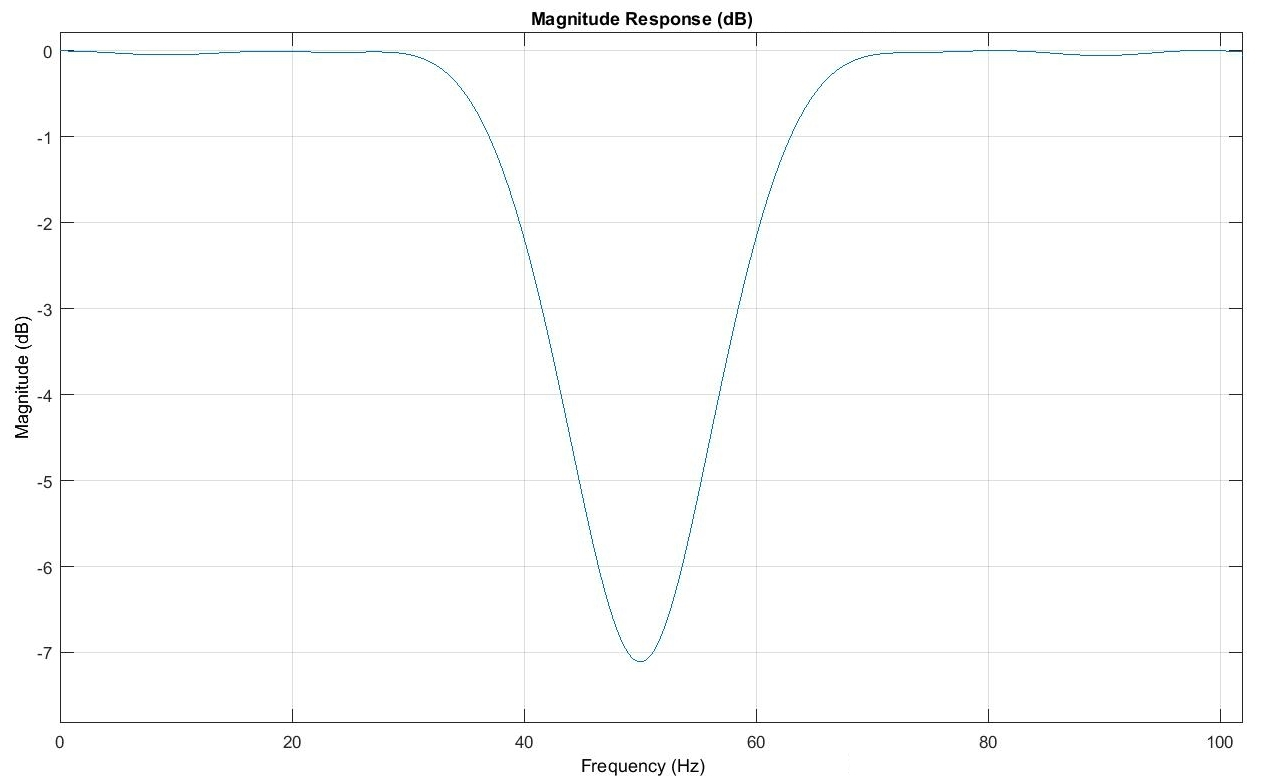
\includegraphics[width=15cm]{FIR_fir1}
    \caption{Respuesta en frecuencia del filtro definido con fir1}
    \label{fig:FIR_fir1}
\end{figure}

Este filtro presenta un comportamiento similar al esperado y un rizado apenas apreciable, pero con un factor de calidad y de rechazo de banda muy bajo. 

Utilizando otra herramienta diseñada por F.S. Schlindwein disponible en el \textit{workshop} de MatLab es posible ajustar aún más el filtro sin apenas esfuerzo. \\
Tras un par de iteraciones el resultado final es el representado en la figura \ref{fig:NOTCH_50Hz}.

\begin{figure} [H]
    \centering
    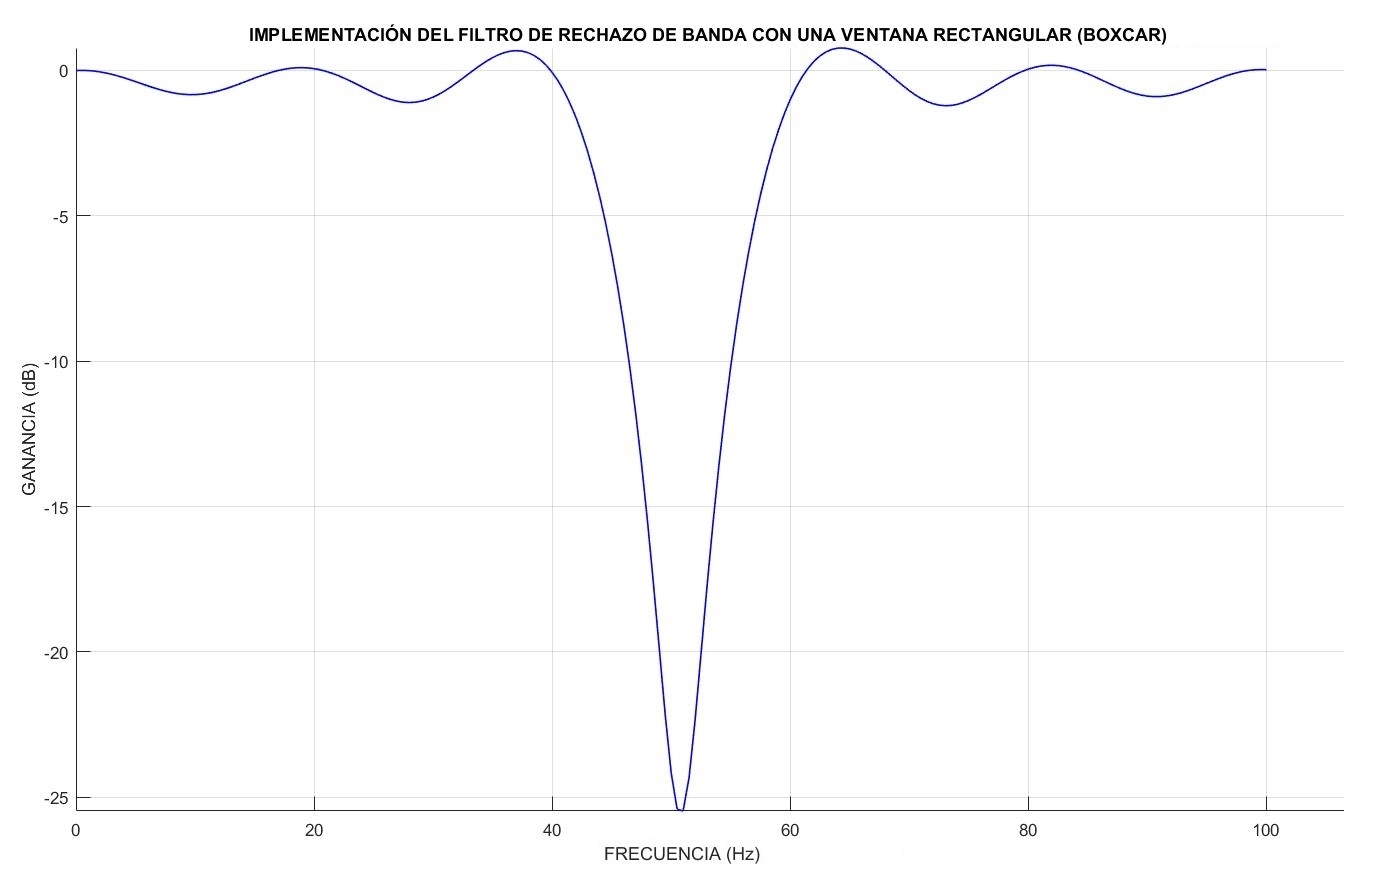
\includegraphics[width=15cm]{NOTCH_50Hz}
    \caption{Respuesta en frecuencia del filtro FIR definido con FIRFILT \cite{FIRFILT}}
    \label{fig:NOTCH_50Hz}
\end{figure}

Este filtro presenta un ancho de banda similar, pero a cambio de introducir un pequeño rizado en la banda deseada, la atenuación a 50 Hz es sensiblemente mayor que en el caso representado en la figura \ref{fig:FIR_fir1}.

El filtrado analógico es inmediato pero muy poco flexible. Utilizando filtros digitales se consigue adaptar el el filtro en función de las necesidades y, en caso necesario, siempre es posible eliminar dicho filtro simplemente cambiando el software. No se debe olvidar que desde el punto de vista del coste/cambio, un cambio a nivel de software casi siempre será mucho más rentable en el producto final que uno a nivel de hardware.

Por desgracia la utilización de esta librería provoca que el código supere las limitaciones de la versión gratuita de Keil haciendo necesaria una licencia para poder compilar.

\clearpage

\subsubsection{Comunicación con la interfaz inalámbrica\label{sec:Software_micro_ESP}}

La transmisión de datos a la interfaz inalámbrica se realiza de forma similar a la ya explicada para comunicar el STM con el ADS. En esta ocasión el STM actuará como Esclavo mientras que el dispositivo que actúa como Master es aquel que hace la función de transmisor de la información. Esto es así debido a las limitaciones impuestas por el ESP12-E. 

En la comunicación con el otro microcontrolador hay tres etapas bien diferenciadas.\\
En la primera la información transmitida son comandos que indican al STM el comportamiento que deberá seguir.\\
La segunda, centrada en la transmisión de pequeñas cantidades de información, no necesita una gran eficiencia en la transmisión. Esta información se utilizará por parte del STM para configurar el ADS.\\
La última fase contempla la transmisión de grandes cantidades de información y por tanto su optimización debe ser máxima.

El código \ref{algoritmo:STM_Transmision_SPI} es el utilizado para transmitir información al ESP y recibirla en caso de que las restricciones de tiempo no sean críticas (primera y segunda fase).

\begin{lstlisting}[label=algoritmo:STM_Transmision_SPI,style = STM-code,frame=single,caption=Transmisión de datos a través de SPI con el STM]
uint8_t commandFromESP(uint8_t command, SPI_HandleTypeDef *hspi1)
{
	uint8_t response = 0x00;	

		HAL_GPIO_WritePin(DRDY_N_GPIO_Port,DRDY_N_Pin, GPIO_PIN_RESET);
		HAL_SPI_TransmitReceive(hspi1, &command, &response, 1, 100);
		HAL_GPIO_WritePin(DRDY_N_GPIO_Port,DRDY_N_Pin, GPIO_PIN_SET);
		HAL_GPIO_TogglePin(LED_GPIO_Port,LED_Pin); 	//LED OFF
		HAL_Delay(50);
	
	return response;
}
\end{lstlisting}

Por la forma en la que está construida la transmisión de datos a través de SPI, la gestión de los pines involucrados directamente en la transmisión la información se realiza de forma automática y es tremendamente eficiente. Sin embargo, la gestión de los pines $\overline{\text{CS}}$ y $\overline{\text{DRDY}}$ se realiza de forma manual y la sincronización entre ambos microcontroladores provoca que la eficiencia de la transmisión se reduzca drásticamente. 

El STM contempla la transmisión de grandes cantidades de información pero, para que esta funcione correctamente, dicha información debe estar en posiciones de memoria consecutivas. Aprovechando esta característica, es posible minimizar el retardo introducido en la sincronización de ambos microcontroladores creando un \textit{buffer} de transmisión de un tamaño lo suficiente grande. De esta forma, cuanto mayor sea la cantidad de datos a transmitir, mayor será la eficiencia de la comunicación.

El código utilizado en la fase 3 es equivalente al código \ref{algoritmo:STM_Transmision_SPI} siendo la única diferencia la cantidad de bytes a transmitir, que es adaptada en función al tamaño del \textit{buffer} de transmisión.

\subsubsection{Programación del microcontrolador\label{sec:Software_micro_ESP}}

Finalmente, tras tener preparado el \textit{firmware} del STM es el momento de cargar dicho código en el microcontrolador. Los microcontroladores de esta familia cuentan con dos métodos para cargar código: usando \textit{jtag} y mediante un \textit{bootloader} embebido.

La primera opción es muy interesante, pues además de programar el microcontrolador da acceso a otras funciones relacionadas con la depuración del código (ejecución en tiempo real, \textit{breackpoints}, visualización de variables, etc). Sin embargo para funcionar es necesario utilizar un hardware específico, y al no disponer de el durante el comienzo del proyecto no se tuvo en cuenta su inclusión durante el desarrollo de la placa.

La segunda opción aprovecha los puertos de UART del microcontrolador para, usando un conversor UART $\leftrightarrow$ USB, programar el STM. Este sistema sólo permite la programación del dispositivo, pero a cambio el hardware extra necesario es mínimo, más teniendo en cuenta que ya se disponía de dicho conversor y, por lo tanto, no fue necesario realizar el desembolso.

\begin{figure} [h]
    \centering
    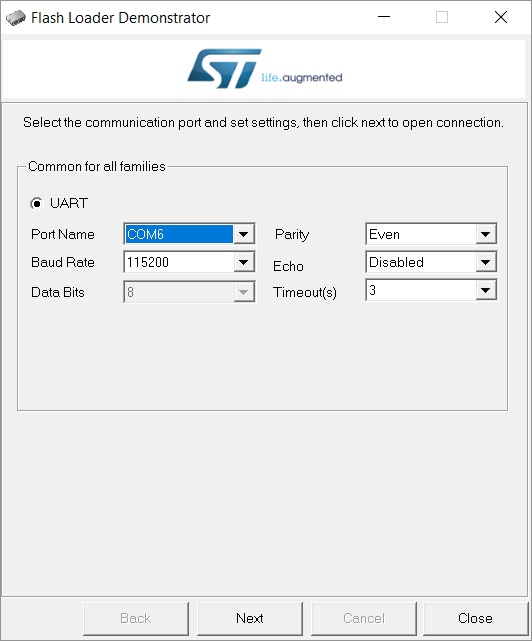
\includegraphics[width=7cm]{STM_prog}
    \caption{Herramienta de programación a través de UART}
    \label{fig:STM_prog}
\end{figure}

Para poder reprogramar el microcontrolador es necesario reiniciarlo mientras se cortocircuitan los pines 1 y 2 del conector preparado para ese fin.

\clearpage

\section{Interfaz inalámbrica\label{sec:Software_inalambrica}}

Los dispositivos integrados en la interfaz inalambrica han sido relegados a una función casi meramente de transmisión pero no se debe olvidar que ambos son microcontroladores y que, por tanto, los dos necesitan ejecutar un \textit{firmware} para funcionar.

Estos dispositivos fueron seleccionados con múltiples objetivos en mente. Por un lado su relación características/coste es muy adecuada, permitiendo crear un sistema final muy completo con un coste muy bajo. Por otro, ambos microcontroladores son compatibles con el IDE de Arduino.

Ser compatible con Arduino \acrshort{IDE} minimiza el tiempo de desarrollo del software, pues el propio IDE realiza la función de abstracción del hardware e incluye un gran número de ejemplos funcionales. Además, al ser ambos dispositivos compatibles, las modificaciones necesarias para portar el código de un microcontrolador a otro son mínimas. Por este motivo a lo largo de este capítulo se expandirá el código implementado en el ESP12-E, quedando el del Bluetooth en segundo plano.

\subsection{Arduino\label{sec:Software_Arduino}}

Arduino fue una iniciativa de Massimo Banzi en 2005 pensada para acercar la electrónica a los estudiantes de un modo sencillo y económico.\\\
Con el paso del tiempo esta plataforma ha ido creciendo, incorporando nuevas placas y microcontroladores, y mejorando tanto en la interfaz como en la comunidad que la respalda.

\begin{figure} [h]
    \centering
    
\includegraphics[width=8cm]{Arduino}
    \caption{Arduino IDE utilizado para la programación del ESP}
    \label{fig:Arduino}
\end{figure}

Por defecto Arduino incluye sólo aquellas placas comercializadas oficialmente por la empresa, pero los desarrolladores han habilitado la posibilidad de crear nuevas librerías e importarlas para que así cualquier persona con suficientes conocimientos pueda añadir las suyas propias.

\clearpage

\subsection{Configuración\label{sec:Software_Arduino_conf}}

Para trabajar con el ESP12-E (esp8266) basta con importar la librería y escoger el componente en el selector de placas integrado.

Las placas no contempladas de forma oficial por Arduino se importan desde File $\Rightarrow$ Preferences.

A continuación se debe introducir la ruta al .json de la librería para que así Arduino tenga un repositorio desde el que buscar aquellas placas que no están instaladas. El resultado final es el mostrado en la figura \ref{fig:Arduino_conf_2}.

\begin{figure} [h]
    \centering
    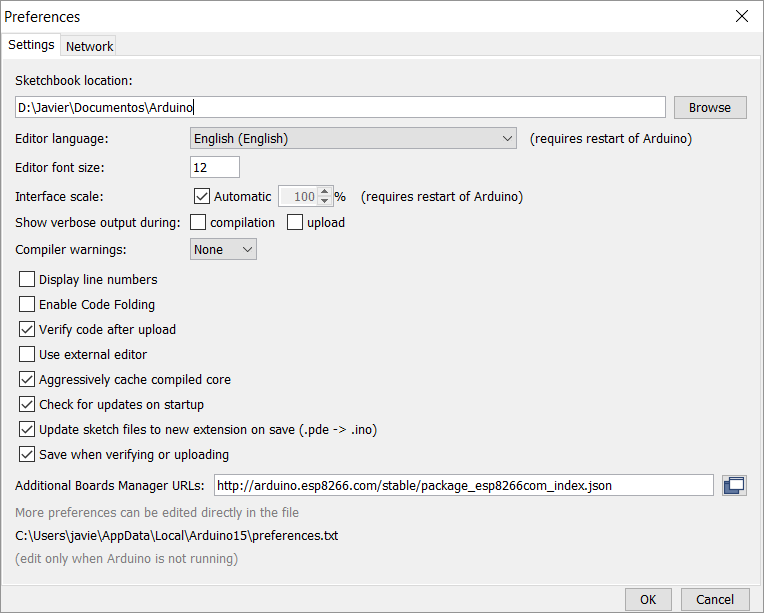
\includegraphics[width=10cm]{Arduino_conf_2}
    \caption{Importar librerías en Arduino}
    \label{fig:Arduino_conf_2}
\end{figure}

Por último se procede a la instalación de las placas deseadas. Para ello se ha habilitado un repositorio con buscador e interfaz gráfica. Este es accesible desde Tools $\Rightarrow$ Board $\Rightarrow$ Boads Manager... 

\begin{figure} [h]
    \centering
    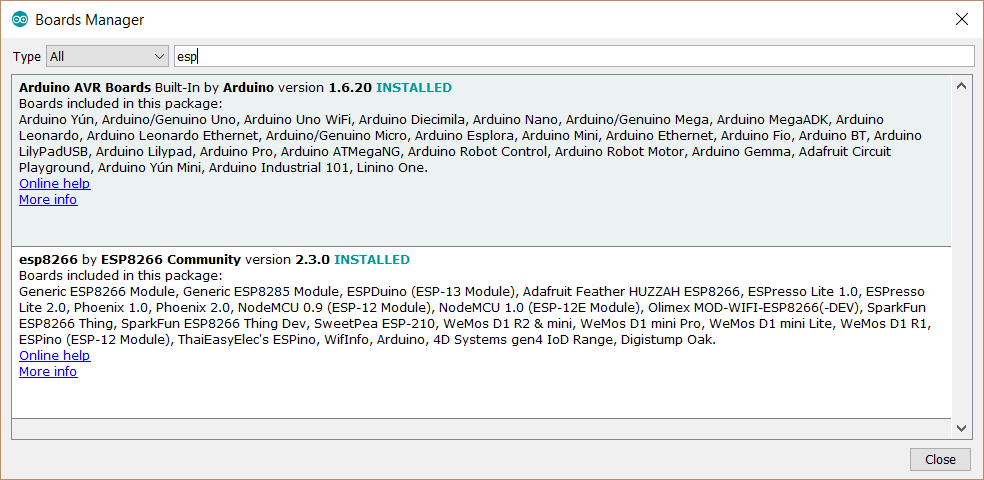
\includegraphics[width=10cm]{Arduino_conf_4}
    \caption{Instalar librerías para nuevas placas}
    \label{fig:Arduino_conf}
\end{figure}

\subsection{Firmware\label{sec:Software_Arduino_firm}}

En los siguientes apartados se detallará el software diseñado para funcionar dentro del microcontrolador. 

\subsubsection{Maquina de estados\label{sec:Software_Arduino_MEstados}}

El código de Arduino está organizado de forma similar al ya explicado para el STM. Este se divide en dos partes, una de \textit{setup} que sólo se ejecuta una vez y otra cíclica denominada \textit{loop}.\\
Para caracterizar el comportamiento del ESP en todo momento se ha creado un sistema de máquina de estados basada en estructuras \textit{switch}/\textit{case} similar al ya explicado para el STM.

En esta ocasión la variable de control principal viene determinada por el sistema de control externo y, en función del estado en el que se encuentre el microcontrolador, este interactúa de una forma u otra con el STM.

\begin{figure} [h]
    \centering
    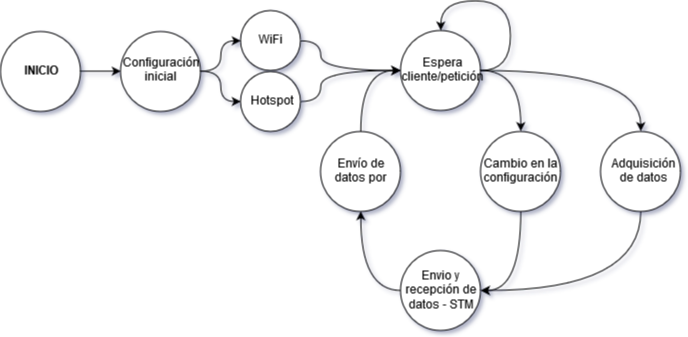
\includegraphics[width=15cm]{Maquina_estados_ESP}
    \caption{Maquina de estados del ESP}
    \label{fig:Maquina_estados_ESP}
\end{figure}

Cada una de las funciones deseadas para el sistema tiene su estado asociado. Además ha sido necesario implementar un sistema de sincronización entre el ESP y el STM que asegure que la transición entre estados de ambos microcontroladores sea siempre simultánea.

\clearpage

\subsubsection{Transmisión de datos por SPI\label{sec:Software_Arduino_Com}}

La transmisión de datos a través de SPI es una de las primeras funciones que los desarrolladores incluyen en las librerías cuando realizan un componente. La librería del ESP8266 no es una excepción y por lo tanto incluye bastantes funciones y definiciones como para poder trabajar de forma cómoda con el ESP en modo Master.

Para funcionar correctamente, eso sí, es necesario conocer perfectamente que pines serán utilizados para la transmisión y configurar tanto los pines como el propio SPI de acuerdo a las necesidades del proyecto.

El ESP cuenta con varios buses SPI. En este proyecto se hace uso de los pines 5 (HSPI\_CLK) , 6 (HSPI\_MISO) y 7 (HSPI\_MOSI) y un GPIO adicional para el $\overline{\text{CS}}$, en esta ocasión el pin 16.

El codigo \ref{algoritmo:ESP_SPI} muestra una configuración funcional de todos los pines así como del SPI.

\begin{lstlisting}[label=algoritmo:ESP_SPI,style = STM-code,frame=single,caption=Configuración de pines para el uso de SPI]
SPI.setClockDivider(SPI_CLOCK_DIV2); //Divides 16MHz clock by 2 to set CLK speed to 8MHz
SPI.setDataMode(SPI_MODE1);  //clock polarity = 0; clock phase = 1 (pg. 8)
SPI.setBitOrder(MSBFIRST);  //data format is MSB (pg. 25)  
  
pinMode(HSPI_CS,OUTPUT);
pinMode(HSPI_CLK,SPECIAL);
pinMode(HSPI_MISO,SPECIAL);
pinMode(HSPI_MOSI,SPECIAL);
pinMode(DRDY_N,INPUT);
pinMode(START,OUTPUT);
\end{lstlisting}

Por simplicidad, a lo largo de todo el proyecto se ha utilizado el mismo modo de funcionamiento del SPI, adaptando el de los microcontroladores al del ADS, pues este viene impuesto por el fabricante mientras que todos los microcontroladores contemplan la utilización de varios modos alternativos.

Cabe destacar del código \ref{algoritmo:ESP_SPI} que el modo de los pines denominado \textsc{ESPECIAL} es característico de aquellos destinados a la transmisión de información. Aunque el pin MISO se considere de entrada, si se configura en modo INPUT la comunicación fallará.

Para transmitir información a través de SPI en cualquier dispositivo de la familia de Arduino (Uno, Due, mega, etc.) se hace uso de la función SPI.transfer() o SPI.transfer16() para datos de 8 o 16 bits respectivamente. \\
Una de las ventajas de Arduino consiste en la estandarización en la medida de lo posible de aquellas funciones que tengan el mismo objetivo y la librería del ESP no es una excepción. Esa misma función y los ejemplos que la acompañan en la referencia oficial para comprender su funcionamiento

\clearpage

La transmisión por SPI desde el STM hacia el ESP se realiza en paquetes de un \textbf{byte}. Para recibir variables tipo \textbf{int} no hay ningún problema, pues al tener ese mismo tamaño se pueden transmitir directamente. Otras variables de mayor tamaño necesitan ser divididas en fragmentos más pequeños para ser transmitidas.

\begin{figure} [h]
    \centering
    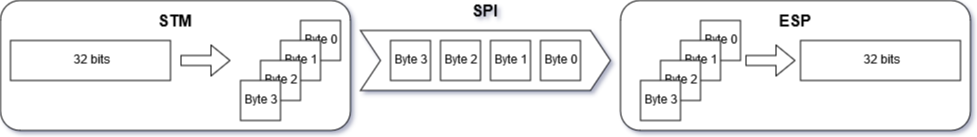
\includegraphics[width=15cm]{Transmision_float}
    \caption{Proceso de división y ensamblado de float para su transmisión}
    \label{fig:Transmision_float}
\end{figure}

Tras recibir los cuatro paquetes de un \textbf{byte} será necesario ensamblarlos para volver obtener la variable original. La misma estructura de datos utilizada para separar los datos en variables independientes se puede usar para revertir el proceso.

\begin{lstlisting}[label=algoritmo:ESP_split_var,style = STM-code,frame=single,caption=Variables y tipos de dato específicos]
union miDato{
 	struct
	{
		byte  b[4];     // Array de bytes de tamaño igual al tamaño de la primera variable: int = 2 bytes, float = 4 bytes
	}split;
	float fval;
} F_recibido; 
\end{lstlisting}

El código \ref{algoritmo:ESP_split_var} es idéntico al usado en el STM para realizar el proceso inverso ya que ambos lenguajes de programación tienen sus bases en \textbf{C}.

Esta operación se repetirá por cada una de las medidas que se realicen.

\clearpage

\subsubsection{Configuración WiFi\label{sec:Software_Arduino_Conf_WiFi}}

El ESP12-E está preparado para trabajar con redes WiFi de 2.4GHz. Para poder funcionar correctamente es necesario configurar aquellos parámetros de red típicos de cualquier conexión Wifi. Estos se ven reflejados en el código \ref{algoritmo:ESP_Wifi_var}.

\begin{lstlisting}[label=algoritmo:ESP_Wifi_var,style = STM-code,frame=single,caption=Variables y tipos de dato específicos]
char ssid[] = "SSID_NAME"; //  your network SSID (name)
char pass[] = "PASSWORD";    // your network password (use for WPA, or use as key for WEP)

IPAddress local_IP(192,168,4,22);
IPAddress gateway(192,168,4,9);
IPAddress subnet(255,255,255,0);
IPAddress remote_IP(192,168,4,121);
\end{lstlisting}
  
El importante que la contraseña de red contenga mínimo 8 caracteres o el sistema no iniciará correctamente.

Una vez configurados los parámetros básicos de comunicación es necesario iniciar la conexión. Para ello es posible iniciar dos modos distintos: conexión a red ya existente o modo \textit{hotspot}.

La conexión a una red ya existente se realiza con el siguiente código durante la fase de configuración del ESP:
  
\begin{lstlisting}[label=algoritmo:ESP_Wifi,style = STM-code,frame=single,caption=Conexión del ESP a una red WiFi ya existente]
// We start by connecting to a WiFi network
Serial.print("Connecting to ");
Serial.println(ssid);
WiFi.begin(ssid, pass)

while (WiFi.status() != WL_CONNECTED) {
	delay(500);
	Serial.print(".");
}
Serial.println("");
  
Serial.println("WiFi connected");
Serial.println("IP address: ");
Serial.println(WiFi.localIP());
\end{lstlisting}

Como se puede apreciar, hasta que la conexión no sea satisfactoria el ESP no arrancará. Tras unos segundos el ESP acaba mostrando por pantalla la dirección IP con la que se ha conectado a la red, IP que debería coincidir con la introducida previamente en el parámetro ``local\_IP''.

Este modo funciona muy bien, permite conexiones rápidas y el consumo de energía es relativamente bajo, pero se hace imprescindible la presencia de una red WiFi ya existente cuyos parámetros sean conocidos.

El modo \textit{Hotspot} es la otra alternativa a este modo. Con esta configuración el ESP hace las funciones de router y punto de acceso, creando una red WiFi de las características deseadas. El código para esto es el mostrado a continuación:

\begin{lstlisting}[label=algoritmo:ESP_Hotspot,style = STM-code,frame=single,caption=Creacion de un punto de acceso en el ESP]
Serial.print("Setting soft-AP configuration ... ");
Serial.println(WiFi.softAPConfig(local_IP, gateway, subnet) ? "Ready" : "Failed!");

Serial.print("Setting soft-AP ... ");
Serial.println(WiFi.softAP("ESPBCI_WIFI", "Password_01", false) ? "Ready" : "Failed!");

Serial.print("Soft-AP IP address = ");
Serial.println(WiFi.softAPIP());
\end{lstlisting}

Este modo dota al ESP de una gran libertad e independencia al eliminar la necesidad de una red WiFi externa, pero la gestión de la información y el consumo de energía se ven perjudicados debido al aumento de carga que recibe el microcontrolador.

Una vez establecida la conexión el ESP se queda en modo de espera de forma indefinida hasta que un nuevo cliente se conecta:

\begin{lstlisting}[label=algoritmo:ESP_Server_handler,style = STM-code,frame=single,caption=Gestión de clientes y peticiones en Arduino]
//########### Server handler #################
// Check if a client has connected
WiFiClient client = server.available();
if (!client) {
	//No client available
	return;
}
\end{lstlisting}

Tras conectarse, el cliente deberá transmitir algún tipo de información. Para evitar el cuelgue del sistema si por algún motivo el cliente no manda datos o la conexión se interrumpe, el ESP espera un tiempo prudencial y si no se ha recibido nada desecha al cliente.

\begin{lstlisting}[label=algoritmo:ESP_Server_handler_2,style = STM-code,frame=single,caption=Gestión de clientes y peticiones en Arduino]
// Wait until the client sends some data
Serial.println("new client");
t1 = millis();
while(!client.available()){
	delay(1);
	Serial.print(".");
	ESP.wdtFeed();    // Evita reinicios por watchdog
	if (millis()-t1 >= 10000){
		Serial.println("Timeout");
		return;
	}
}
\end{lstlisting}

Por último se interpreta la información almacenándola en una variable para su posterior utilización.

\begin{lstlisting}[label=algoritmo:ESP_Server_handler_2,style = STM-code,frame=single,caption=Gestión de clientes y peticiones en Arduino]
// Read the first line of the request
String req = client.readStringUntil('\r\n');
\end{lstlisting}

Todos los microcontroladores tienen un sistema de control llamado \textbf{Watchdog} que monitoriza el estado del microcontrolador. Si detecta que el dispositivo lleva demasiado tiempo en un bucle este se activa y realiza un reinicio de emergencia. 

El ESP cuenta con dos tipos distintos de Watchdog, uno accionado por software y otro por hardware. El primero se activa en caso de que el programa funcione correctamente y se haya producido un bucle no deseado o no contemplado. El segundo lo hace en caso de fallo total del sistema. Para evitar que en ciertas partes del código en las que el ESP se queda esperando de forma indefinida se active el whatchdog por software es necesario introducir la siguiente línea:
\begin{lstlisting}[label=algoritmo:ESP_Server_wdt,style = STM-code,frame=single,caption=Reinicios por \textit{watchdog}]
ESP.wdtFeed();    // Evita reinicios por watchdog
\end{lstlisting}
De esta forma el contador que utiliza para monitorizar el tiempo que lleva en el bucle inicializa y se evita un reinicio indeseado.

\subsubsection{Transmisión de datos a través de WiFi\label{sec:Software_Arduino_Com_WiFi}}

Una vez se ha establecido la conexión entre ambos dispositivos es el momento de transmitir información. Arduino cuenta con varias funciones asociadas a la gestión de la información tanto a nivel servidor como a nivel cliente, todas ellas englobadas dentro de la librería ``WIFI''.

Si se desea usar el protocolo TCP la utilización de client.print resulta altamente tentadora. Esta estructura presenta ciertos paralelismos con Serial.print y permite además la interpretación del valor directamente al realizar una representación en formato comprensible para los humanos.
 
Sin embargo, al utilizar esta función se realiza también una conversión de la variable a otro formato junto con su correspondiente pérdida de precisión y cambio en el tamaño. La siguiente tabla ilustra con ejemplos los resultados de estas transformaciones si se representan con 5 dígitos de precisión.
\begin{table} [H]
	\centering
	\begin{tabular}{|c|c|c|}
\hline 
\textbf{Valor real} & \textbf{Representación} & \textbf{Tamaño [bits]} \\ 
\hline 
1 & 1 & 8 \\ 
\hline 
$1.\wideparen{3}$ & 1.33333 & 56\footnotemark \\ 
\hline 
	\end{tabular} 
	\caption{Representación de datos usando client.print()}
	\label{tab:client_print_rep}
\end{table}
\footnotetext{{(n*enteros + 1 (punto) + k*decimales)}}

Al tratar con variables en las que los decimales contienen una gran cantidad de información, el uso de la función client.print() queda completamente descartado, pues provoca una pérdida de precisión muy alta o un aumento drástico del espacio ocupado en memoria por cada medida.

Una alternativa a esta función es client.write(). Esta es capaz de transmitir 8 bits o un fichero de datos del cliente al servidor, independientemente de la representación de esos datos.\\
Este sistema es menos intuitivo pero a cambio evita pérdida de precisión y asegura que los datos transmitidos conservarán su integridad, tanto de valor como de tipo de variable y tamaño.

La transmisión a través de TCP está orientada a asegurar que los datos llegarán sin errores a costa de disminuir la velocidad efectiva. 

En un intento de mejorar la velocidad de transmisión se ha explorado la utilización de UDP usando las funciones udp.beginPacket(), udp.write() y udp.endPacket().\\
Los resultados se presentan en el capítulo \ref{sec:Resultados}, pero su inclusión al sistema ha sido desechada porque el ahorro de tiempo no es muy destacable y en cambio en función de las condiciones de la red, la cantidad de paquetes perdidos puede resultar demasiado elevada.

\clearpage

\section{LabView\label{sec:Software_Labview}}

El sistema en este punto puede hacer uso de cualquier ordenador o \textit{smartphone} como interfaz. Por comodidad, se ha escogido LabView como entorno de prototipado para la interfaz, ya que incluye un gran número de funciones y elementos gráficos que simplifican el desarrollo de un proyecto y permite generar un ejecutable que funcione en cualquier ordenador, tenga o no instalada una versión de LabView.

\begin{figure} [h]
    \centering
    
\includegraphics[width=7cm]{LabView}
    \caption{Logotipo de LabView}
    \label{fig:LabView}
\end{figure}

\subsection{Interfaz gráfica\label{sec:Software_Labview_interfaz}}

Desde LabView se han habilitado funciones para la representación de la información recibida desde el sistema de adquisición de datos. En una versión inicial contiene aquellos elementos necesarios para comprobar que todo funciona correctamente y representar las señales recibidas.

\begin{figure} [h]
    \centering
    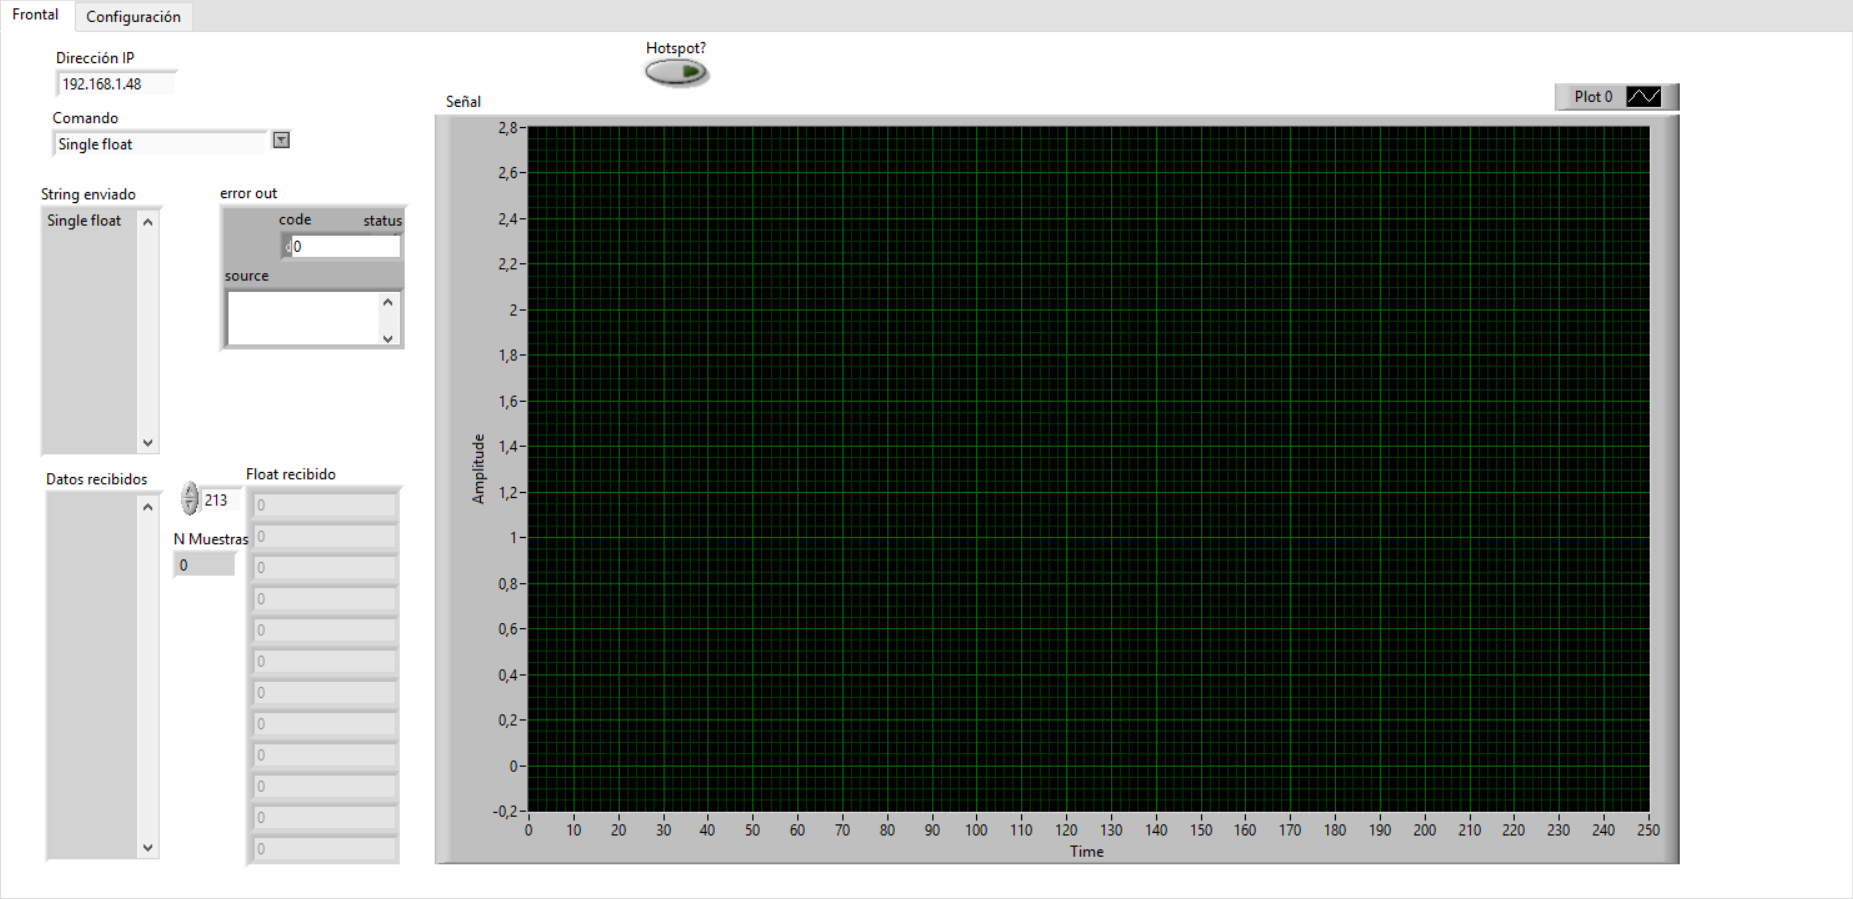
\includegraphics[width=16cm]{Labview_interfaz}
    \caption{Interfaz de LabView: Representación de la información}
    \label{fig:Labview_interfaz}
\end{figure}

Como se puede apreciar en la imagen \ref{fig:Labview_interfaz}, la interfaz está organizada en pestañas.\\
La primera presenta los datos recibidos, los enviados y otros elementos de control.\\
La segunda contiene todos los elementos necesarios para modificar los parámetros de configuración del ADS.

\begin{figure} [h]
    \centering
    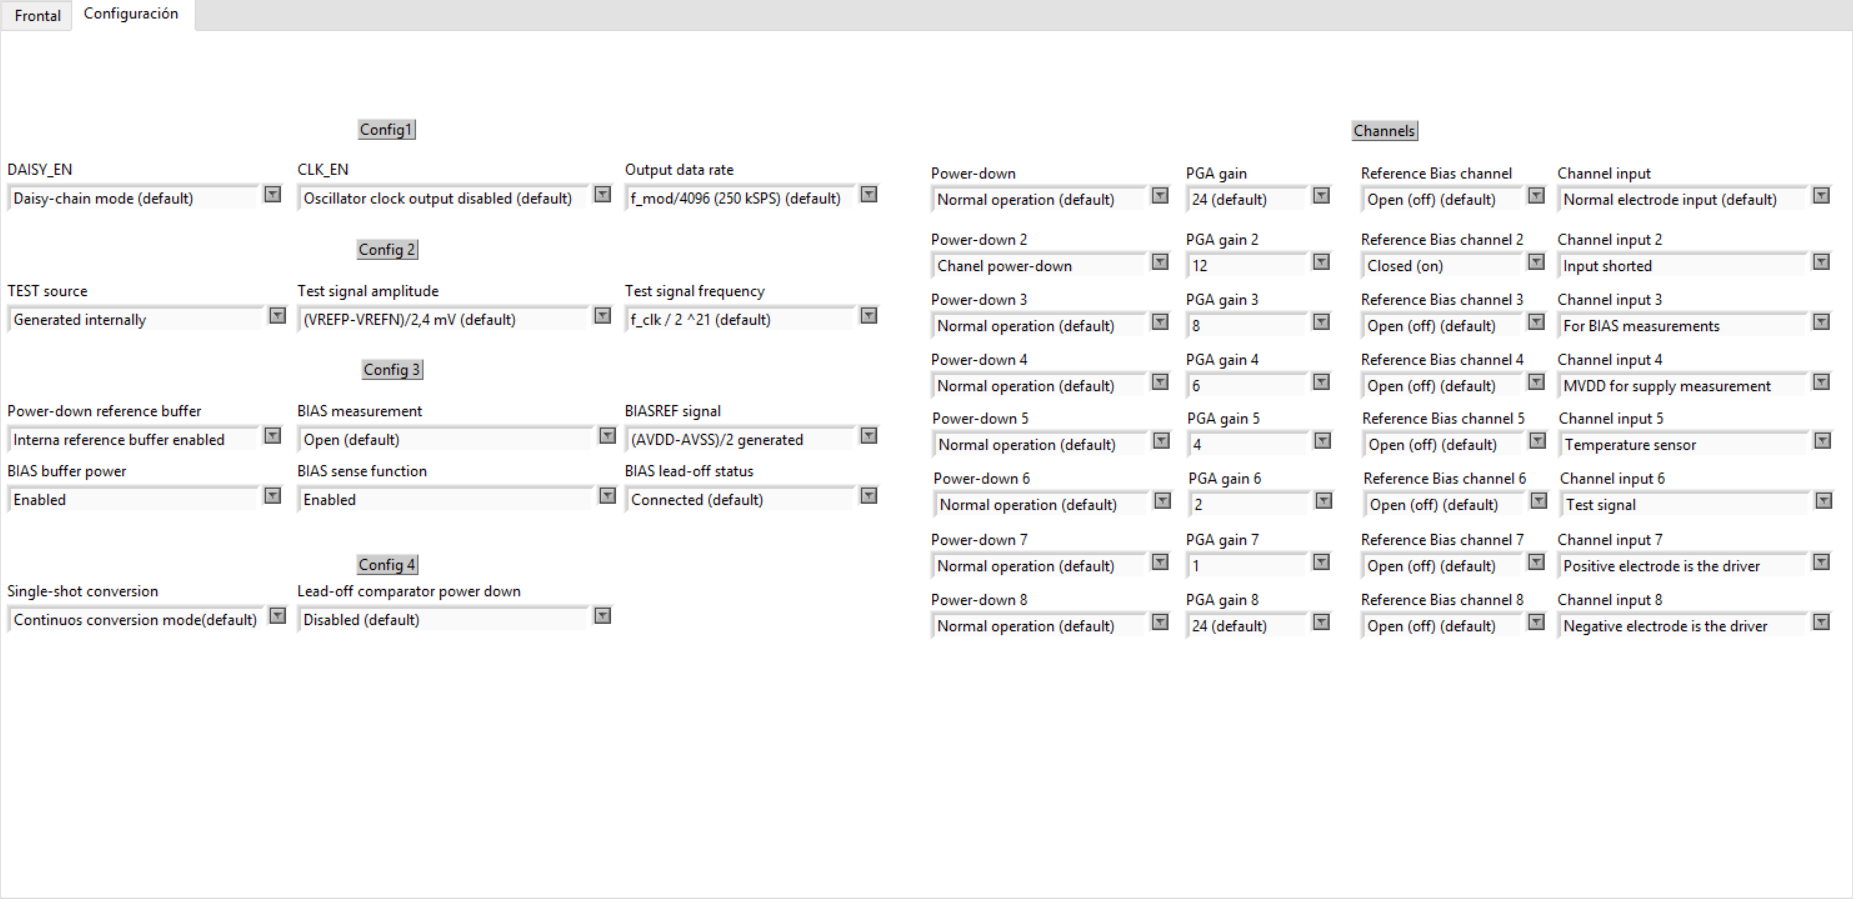
\includegraphics[width=16cm]{Labview_interfaz_2}
    \caption{Interfaz de LabView: Configuración del ADS}
    \label{fig:Labview_interfaz_2}
\end{figure}

La figura \ref{fig:Labview_interfaz_2} muestra todos los parámetros del ADS, estando dispuesta la configuración de los canales de forma que se puedan ver todas las opciones disponibles.

Esta interfaz ha sido desarrollada por parte de la alumna Nerea Urrestarazu durante la realización de su Trabajo fin de Máster y cedida con el objetivo de ahorrar tiempo. El archivo .vi ha sido utilizado como base, conservando la distribución y elementos básicos relacionados con los registros y funciones del ADS mientras que la lógica ha sido rehecha para cumplir con las necesidades de este proyecto.

La lógica consta de varias partes, por un lado una encargada de transmitir y recibir información desde la red WiFi a la que esté conectado el ordenador. Por otro lado, otra cuya función es construir la orden que se desea transmitir a la placa adquisidora. Finalmente, tras recibir la contestación de la placa, esta se interpreta realizando las acciones pertinentes en función del significado, normalmente almacenado y representación de las mediciones.

\clearpage

\subsection{Comunicación WiFi\label{sec:Software_Labview_WiFi}}

El envío y recepción de los datos en el PC ha sido implementado de dos maneras: por TCP y por UDP. 

La figura \ref{fig:Labview_Transmision_TCP} muestra una representación simplificada de los bloques necesarios para la transmisión por TCP. Con esta configuración el ordenador inicia la conexión, manda una petición al ESP indicando que se desean medir datos y espera hasta que se reciba un paquete que contenga la cadena de caracteres retorno de carro seguida de nueva linea (\textbackslash r\textbackslash n).

\begin{figure} [h]
    \centering
    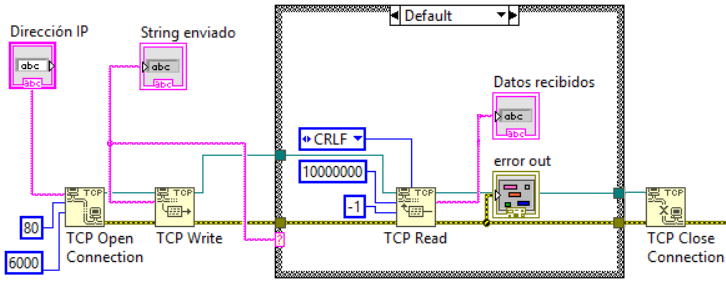
\includegraphics[width=15cm]{Transmision_TCP}
    \caption{LabView: Transmisión y recepción de datos a través de TCP}
    \label{fig:Labview_Transmision_TCP}
\end{figure}

En caso de que la comunicación se cierre por parte del ESP o por un error de red se genera un evento de error que será gestionado por el siguiente conjunto de bloques y mostrado al usuario sin interrumpir el resto del programa.

\begin{figure} [h]
    \centering
    \includegraphics[width=9cm]{Labview_error}
    \caption{Bloques para ignorar errores conocidos}
    \label{fig:Labview_error}
\end{figure}

\subsection{Conversión de datos\label{sec:Software_Labview_ConvDatos}}

Los datos se reciben en un \textbf{string} de longitud igual a cuatro veces el total de los datos medidos y si estos son representados directamente resultan ilegibles. Para poder obtener los datos originales es imprescindible realizar una división cada cuatro bytes y reinterpretar los valores como \textbf{float} con el bloque \textit{cast}. En la figura \ref{fig:LabView_convertir_datos} se muestran los bloques encargados de realizar esta función.

\begin{figure} [h]
    \centering
    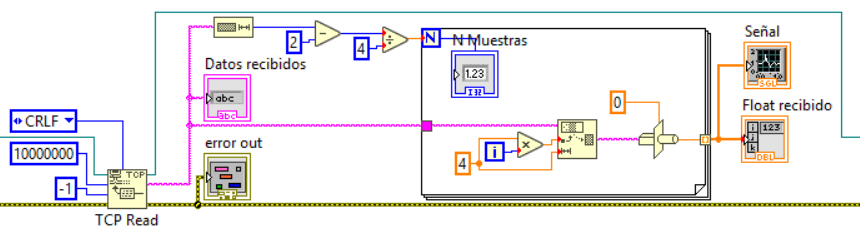
\includegraphics[width=15cm]{LabView_convertir_datos}
    \caption{Extracción y conversión de datos}
    \label{fig:LabView_convertir_datos}
\end{figure}

Estos bloques están pensados para funcionar independientemente del número de muestras adquiridas, aportando mayor flexibilidad al diseño.

\subsection{Alternativa UDP\label{sec:Software_Labview_AltUDP}}

Como se ha mencionado anteriormente, se ha trabajado en una alternativa que aprovecha las ventajas del UDP para transmitir la información hacia el ordenador. Los bloques utilizados para realizar esta función los siguientes:

\begin{figure} [h]
    \centering
    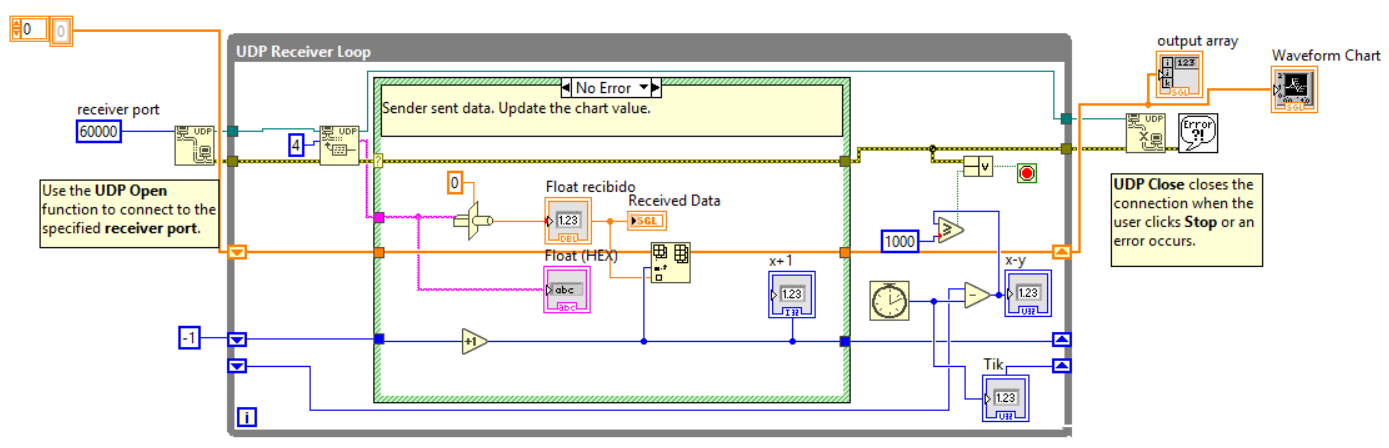
\includegraphics[width=15cm]{LabView_UDP}
    \caption{Recepción de datos a través de UDP}
    \label{fig:LabView_UDP}
\end{figure}

Este sistema funciona de forma similar al equivalente en TCP. En esta ocasión que en lugar de esperar a un caracter concreto para dar la comunicación por concluida esta se cierra tras un tiempo de espera sin recepción de datos. De esta forma se evita un bloqueo en caso de que se pierda alguna muestra.